% -*-latex-*-

\chapter{The Experiment}
\label{C5}

E08-027 was conducted in Hall A at Thomas Jefferson National Accelerator Facility (Jefferson Lab or JLab) from March to May, 2012. The experiment was a precise measurement of the inclusive polarized cross-section for electron scattering from protons. The main goal of this experiment is to extract the proton spin-dependent structure function $g_2$ in the resonance region with $0.02<Q^2<0.20$ GeV${}^2$ \cite{G2P}. The measured $g_2^p$ data will allow us to extract the longitudinal-transverse spin polarizability $\dlt$ for the proton to perform a benchmark test of $\chi$PT predictions and to test the BC sum rule as we already discussed in \Cref{C4}.

During E08-027, a longitudinally polarized electron beam was scattered from a transversely polarized proton target to measure the transverse polarized cross-section differences $\Delta\sigma_\perp$. The Hall A High Resolution Spectrometers (HRS) were used to detect the scattered electrons at an angle of \SI{5.77}{\degree}. The $\Delta\sigma_\perp$ data were combined with the longitudinal polarized cross-section differences $\Delta\sigma_\parallel$ from JLab Hall B EG4 experiment \cite{EG4} in the same kinematic region to extract the proton $g_2$ structure function. The $\Delta\sigma_\parallel$ data was also collected in E08-027 with a longitudinally polarized proton target at a 2.254 GeV incident beam energy to verify the EG4 data.

\begin{figure}[tb!]
  \centering
  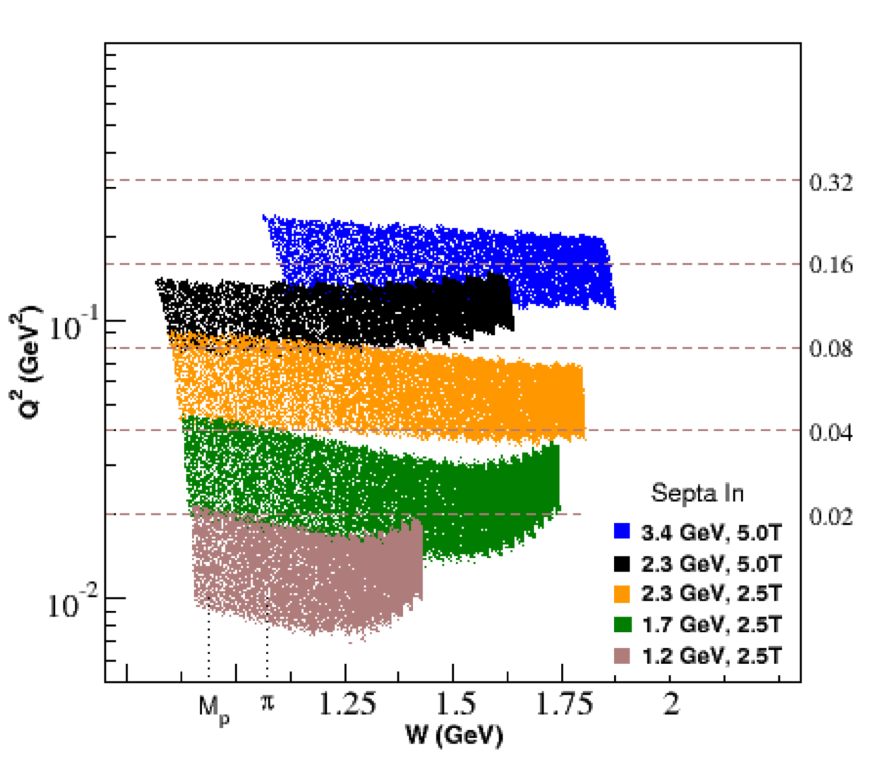
\includegraphics[width=0.75\textwidth]{figs/kinematics-g2p.png}
  \caption[Kinematic coverage of E08-027.]{Kinematic coverage of E08-027. The legend shows the beam energy and target field strength for each setting. Plot reproduced from \cite{G2P}. \label{C5F1}}
\end{figure}

\begin{table}[tb!]
  \centering
  \newcolumntype{C}[1]{>{\centering\arraybackslash}m{#1}}
  \begin{tabular}{|c|C{2.5cm}|C{2cm}|C{2cm}|C{2.5cm}|}
    \hline
      & Beam Energy (GeV) & Field Strength (T) & Field Angle & Septum \\ \hline
    1 & 2.254 & 0.0 & N/A & 48-48-16 \\ \hline
    2 & 2.254 & 2.5 & \SI{90}{\degree} & 48-48-16 \\ \hline
    3 & 2.254 & 2.5 & \SI{90}{\degree} & 40-32-16 \\ \hline
    4 & 1.710 & 2.5 & \SI{90}{\degree} & 40-00-16 \\ \hline
    5 & 1.157 & 2.5 & \SI{90}{\degree} & 40-00-16 \\ \hline
    6 & 2.254 & 5.0 & \SI{0}{\degree} & 40-00-16 \\ \hline
    7 & 2.254 & 5.0 & \SI{90}{\degree} & 40-00-16 \\ \hline
    8 & 3.350 & 5.0 & \SI{90}{\degree} & 40-00-16 \\ \hline
  \end{tabular}
  \caption[Beam energy and target field configurations.]{Beam energy and target field configurations for E08-027. The septum configuration is also listed in this table. During the experiment, the spectrometers were set at \SI{5.77}{\degree}. \label{C5T1}}
\end{table}

The data were acquired in four different beam energies between 1.157 and 3.350 GeV and two different target field strength configurations (2.5 T and 5.0 T). The kinematic coverage of each setting is shown in \Cref{C5F1}. Only those settings with the transverse target field are included in the figure. Since the minimum scattering angle limit of the HRS is \SI{12.5}{\degree} \cite{Alcorn2004}, a septum magnet was installed in front of the spectrometer pair to bend the $\approx$\SI{5.77}{\degree} scattered electrons into the HRS. Unfortunately, portions of the septum magnet coils were burned twice during the experiment, which led to three different septum configurations. The experiment configurations are summarized in \cref{C5T1}.

The polarized proton in E08-027 was provided by a frozen ammonia target. The Dynamic Nuclear Polarization (DNP) process was used to polarize the target. Beam current was limited to 50 nA during the experiment to reduce the depolarization of the target. However, the standard Hall A beamline electronics were not designed to work with such low beam currents. For E08-027, new beam current monitors, beam position monitors and chicane were used to accommodate the target. These will be presented in \Cref{C5S2}.

This chapter will discuss the electron beam, the Hall A beamline components, the polarized ammonia target and the HRS system.

\section{The Electron Accelerator}
\label{C5S1}

\subsection{Continuous Electron Beam Accelerator Facility}
\label{C5S1SS1}

The superconducting radio-frequency Continuous Electron Beam Accelerator Facility (CEBAF) at JLab consists of a polarized electron source, an injector, two linacs, two recirculation arcs and extraction elements to send the beam into three experimental halls: A, B and C \footnote{Following the 12 GeV upgrade of Jefferson lab, which was carried out after this experiment, a fourth experimental hall, Hall D, was added.} \cite{Sulkosky2007}. \Cref{C5S1SS1F1} is a sketch of the CEBAF accelerator.

\begin{figure}[tb!]
  \centering
  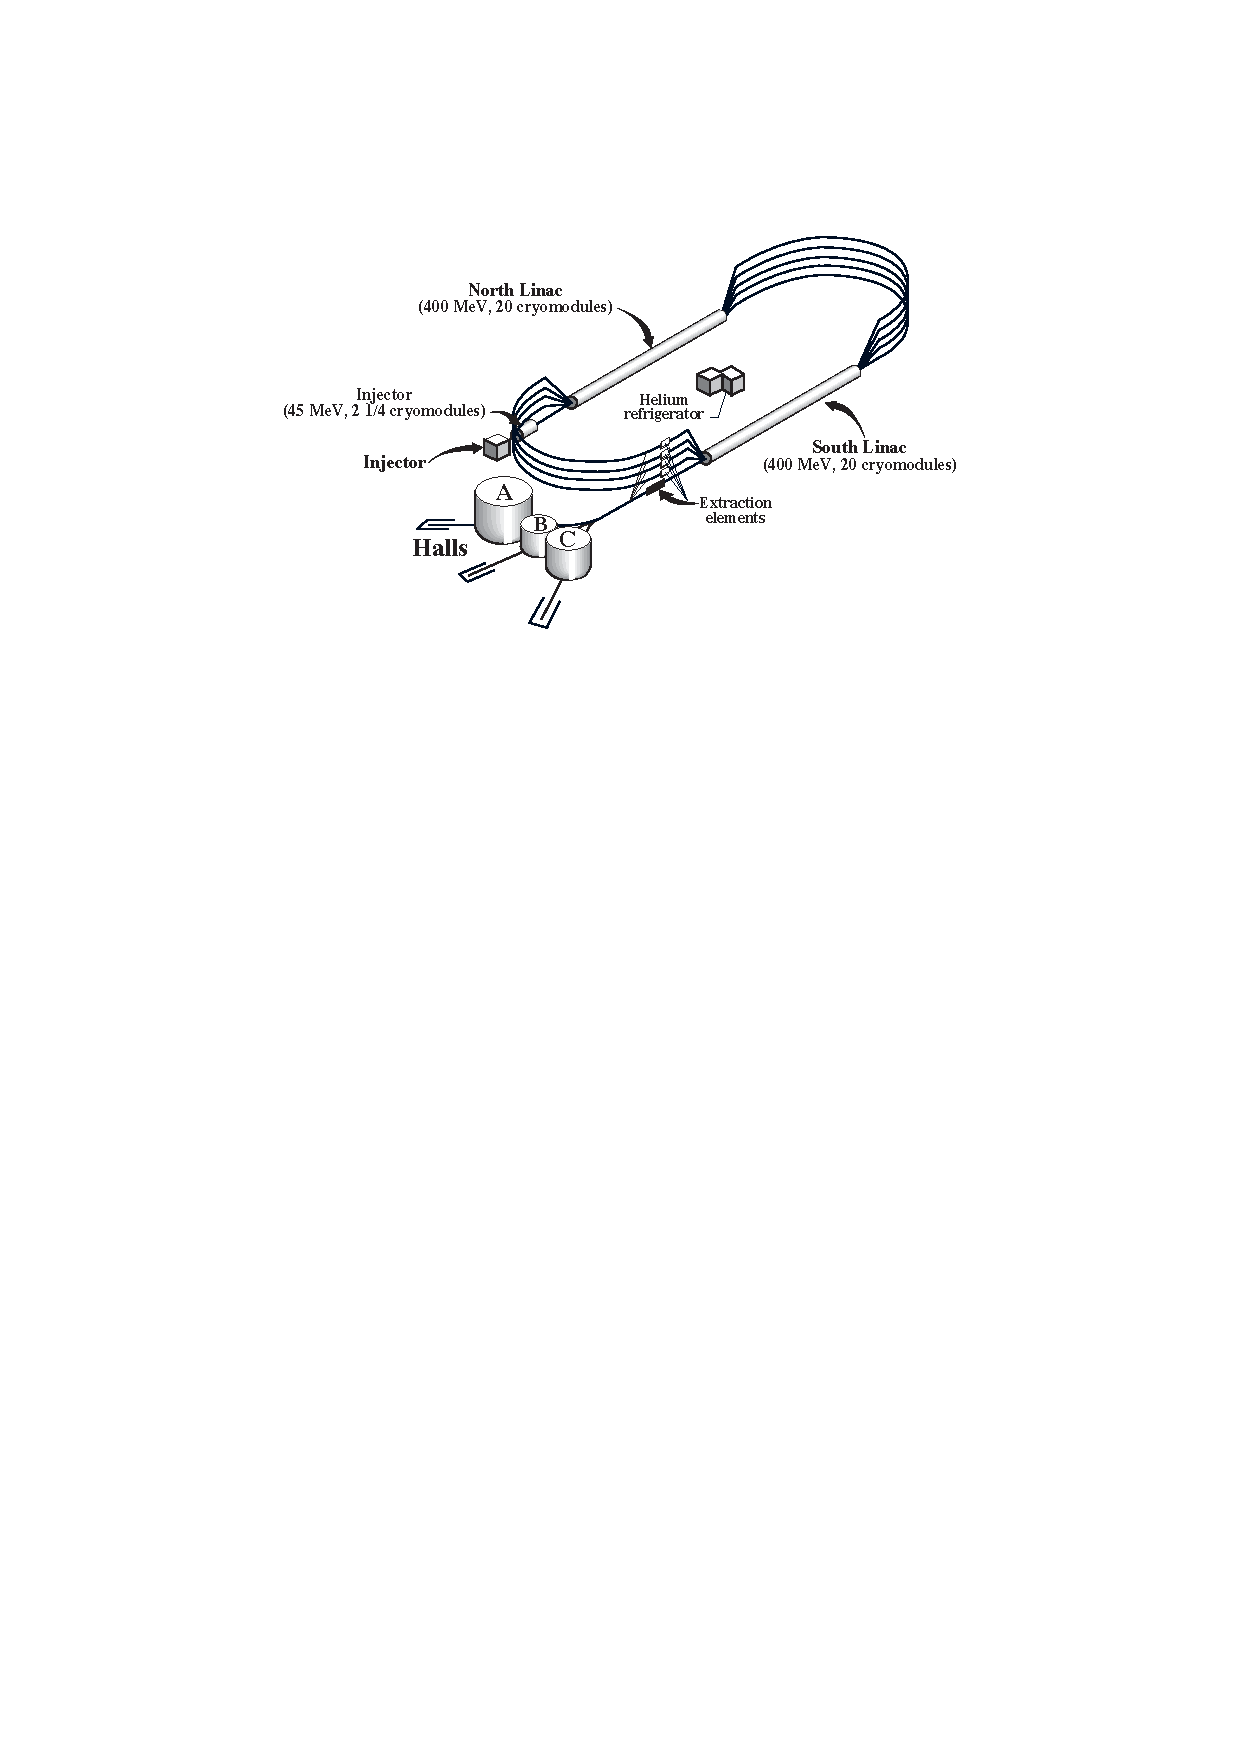
\includegraphics[width=0.7\textwidth]{figs/accelerator.pdf}
  \caption[Sketch of the CEBAF accelerator.]{Sketch of the CEBAF accelerator during the 6GeV era. The beam travels once through the North and South linacs with each recirculation, when part of it could be extracted to any of the three Halls. The linac energies shown are for operation at 4 GeV; at 6 GeV each linac operates at 600 MeV. Plot reproduced from \cite{Gross2011}. \label{C5S1SS1F1}}
\end{figure}

Once the electron beam is generated, it is injected into the accelerator after an initial acceleration to 45 MeV. A Wien filter is used at the injector to set the polarization angle of the electrons. The precession of the electrons is taken into account to assure that the electrons are longitudinally polarized when they reach the experimental halls. As shown in \Cref{C5S1SS1F1}, the main acceleration part is composed of two anti-parallel linacs linked by nine recirculation arcs for up to five passes. Each linac can be used to accelerate electrons for all passes since the electrons are ultra-relativistic and travel at almost the same speed. At the end of the second linac, the beam can either enter the recirculation arc to be accelerated one more pass or be extracted into the experimental halls.

CEBAF can provide electron beams at different but correlated energies to three experimental halls simultaneously. Although the accelerator was originally designed to be operated with a maximum beam energy around 4 GeV, the maximum achieved beam energy reached nearly 6 GeV with the state-of-art superconducting radio-frequency technologies. The maximum total beam current available among the three halls is 200 $\mu$A. The current can be split arbitrarily between three inter-leaved 499 MHz bunches. Each of the bunches can then be peeled off to send beam to one of the halls \cite{Sulkosky2007}. CEBAF has provided electron beams at 1-150 $\mu$A for experimental Hall A and C and 1-100 nA for experimental Hall B since 2000.

\subsection{Beam Helicity}
\label{C5S1SS2}

At Jefferson Lab, the polarized electron beam is produced by illuminating a GaAs photocathode with circularly polarized photons \cite{Gross2011}. The beam helicity needs to be reversed to measure helicity-dependent observables like the cross-section differences in E08-027. The spin of the photo-emitted electron is correlated to the circular polarization state of the photon. It can be either aligned parallel (1 or +) or anti-parallel (0 or -) to the electron momentum direction, which are the two helicity states of the electron. Thus the beam helicity can be reversed by changing the polarization state of the light.

\begin{figure}[b!]
  \centering
  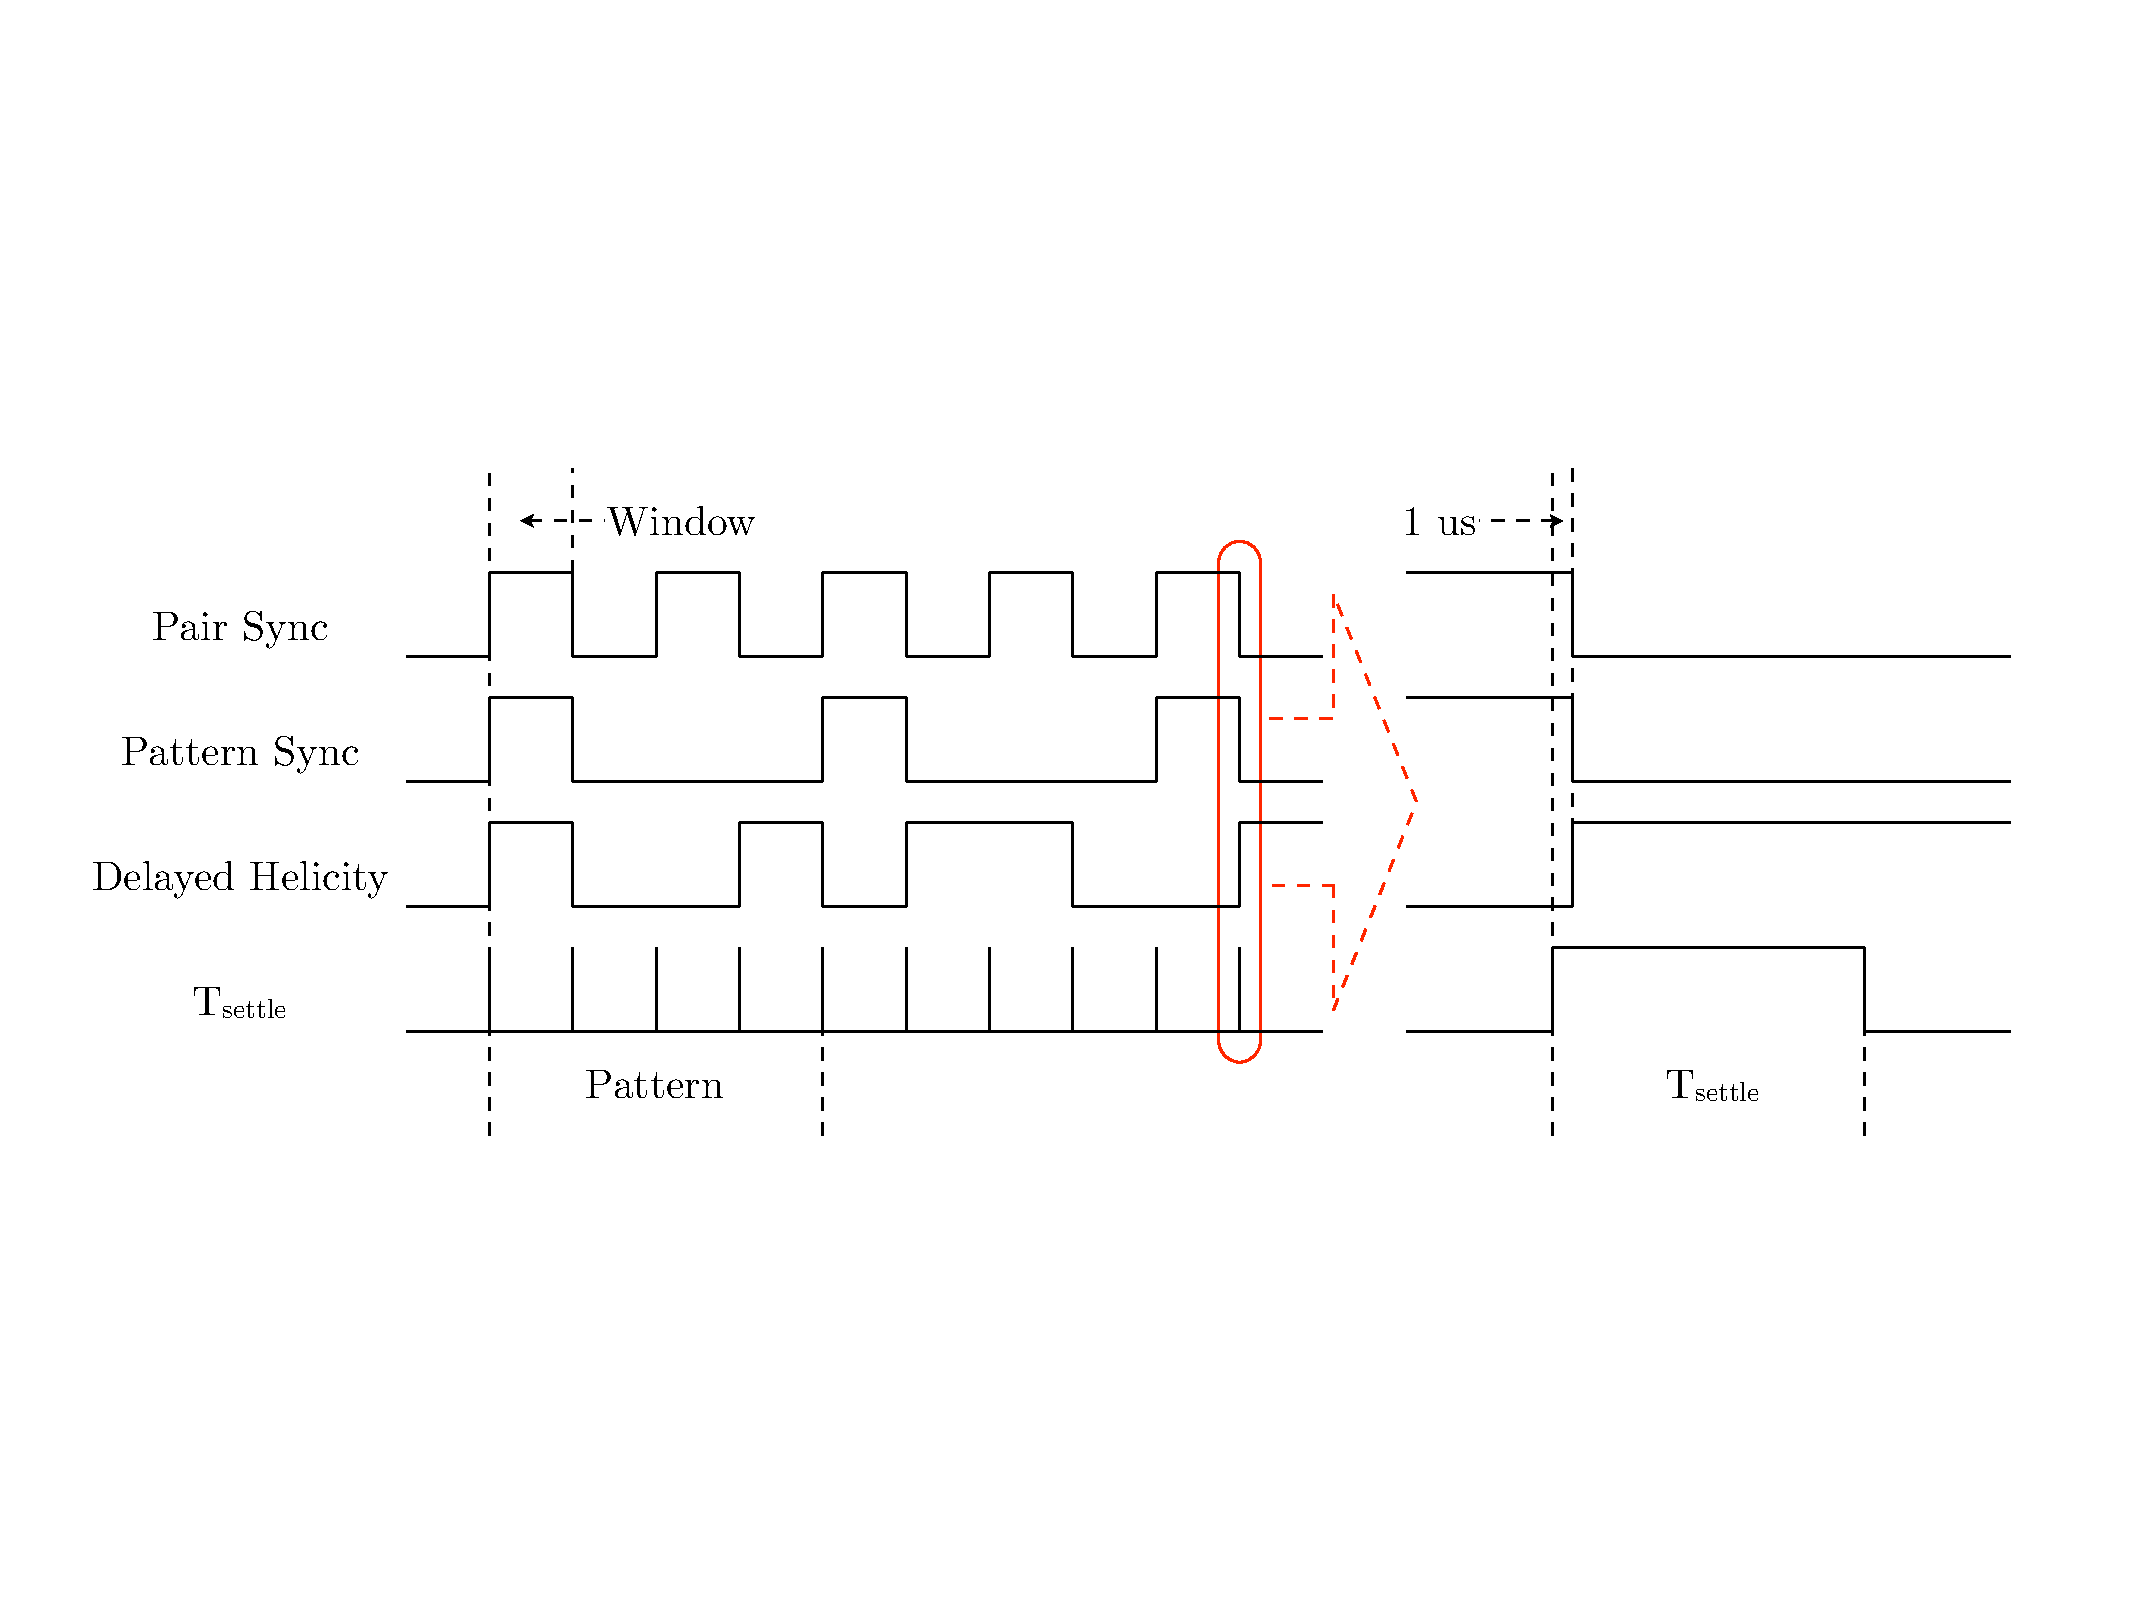
\includegraphics[width=\textwidth]{figs/helicity-signal.pdf}
  \caption[Helicity signals received by experiment DAQ.]{Helicity signals received by experiment DAQ. The right side shows the time sequence of these signals, notice that the $\tsettles$ signal is 1 $\mu$s prior to the other three to avoid misalignment. \label{C5S1SS2F1}}
\end{figure}

A programmable logic generator known as the Helicity Control Board is installed at the injector to control the helicity of the electron beam \cite{Flood2010}. It generates a logic signal known as the Helicity Flip signal to control the polarity of the high voltage of the Pockels Cell on the Laser Table in the injector. The Pockels Cell is a crystal that acts as a quarter-wave retardation plate when a high voltage is applied on it. Flipping the polarity of the high voltage of the Pockels Cell changes the circular polarization state of the laser and hence changes the helicity of the electron beam \cite{Hansknecht2007}. Since there is no mechanical movement, the Pockels Cell can be used to provide relatively fast reversal of the beam helicity. Normally, the beam helicity is flipped at 30 Hz. However during E08-027, the helicity was flipped at 960.02 Hz to be compatible with other experimental halls.

The actual sequence of the beam helicity is a series of identical length helicity windows in which helicity is stable. See \Cref{C5S1SS2F1}. To minimize the low frequency systematic uncertainty, the helicity signal always shows up in some symmetric multi-window patterns, like a double-window Pair or a four-window Quartet. For example, the helicity sequence in a Quartet pattern can either be ($+--\,+$) or ($-++\,-$) so any linear background is cancelled out.

The helicity of the first window of each pattern is determined by a pseudo-random generator in the Helicity Control Board. Any correlation between the helicity of the beam and other data acquisition (DAQ) components is removed by using this pseudo-random generator. To minimize any other possible systematic effects, the helicity signal received by experiment DAQ is delayed by 8 helicity windows. However, the actual helicity of the incident electrons can still be extracted since the pseudo-random algorithm is fully known.

Due to the non-zero response time of the Pockels Cell to the HV change, the helicity during the transition time between two helicity windows is not stable. A $\tsettles$ signal is generated to deal with this problem. This signal is composed by a $\tsettle$ part and a $\tstable$ part. $\tsettle+\tstable$ equals to the time length of a helicity window and the $\tsettle$ is chosen to be slightly longer than the transition time of the Pockels Cell.

Aside from the Delayed Helicity and the $\tsettles$ signal, the experiment DAQ also receives two more signals from the Helicity Control Board. The Pattern Sync signal indicates the start of a helicity pattern with a logic 1 and remains 0 in other helicity windows. The Pair Sync signal begins with a logic 1 at the first window of a helicity pattern and then toggles between 0 and 1. These two signals are useful to help predicting the actual helicity. \Cref{C5S1SS2F1} shows the relations of these signals and their time sequence.

The helicity scheme generated by the Helicity Control Board can be varied. During E08-027, the helicity pattern was set to be Quartet. The $\tsettle$ and $\tstable$ was set to 70 $\mu$s and 971.65 $\mu$s respectively so the helicity reversal rate is 960.02 Hz. However the typical DAQ rate of E08-027 was $5\sim6$ kHz. The existing helicity decoder to extract the actual helicity from the Delayed Helicity signal did not work at this DAQ rate. A new helicity decoder was designed for E08-027. The algorithm and the test of this new helicity decoder is discussed in \Cref{A1}.

An insertable half-wave plate (IHWP) located upstream of the Pockels cell could also be used to reverse the beam helicity manually. Insertion of the half-wave plate was performed several times per day to check and to help cancel the helicity dependent systematic effects.

\section{Hall A Beamline}
\label{C5S2}

As we mentioned at the beginning of this chapter, beam current of E08-027 was limited to 50 nA due to the depolarization effect of the target. Thus new beam current monitors (BCMs) and beam position monitors (BPMs) which could work at very low beam currents were used in this experiment to accommodate the target. To further reduce the depolarization effect, a pair of slow rasters were installed in Hall A for the first time to spread the beam over the target uniformly. Since the strong transverse target field would bend the incident and the scattered electrons, two chicane dipole magnets were installed in Hall A upstream of the target to compensate the effect of the target field. A local beam dump was also installed downstream of the target to stop the electron beam when it could not reach the standard beam dump of Hall A due to the effect of the target field. \Cref{C5S2F1} is a schematic diagram indicating major experimental components of E08-027. These new instruments will be presented in this section.

\begin{figure}[b!]
  \centering
  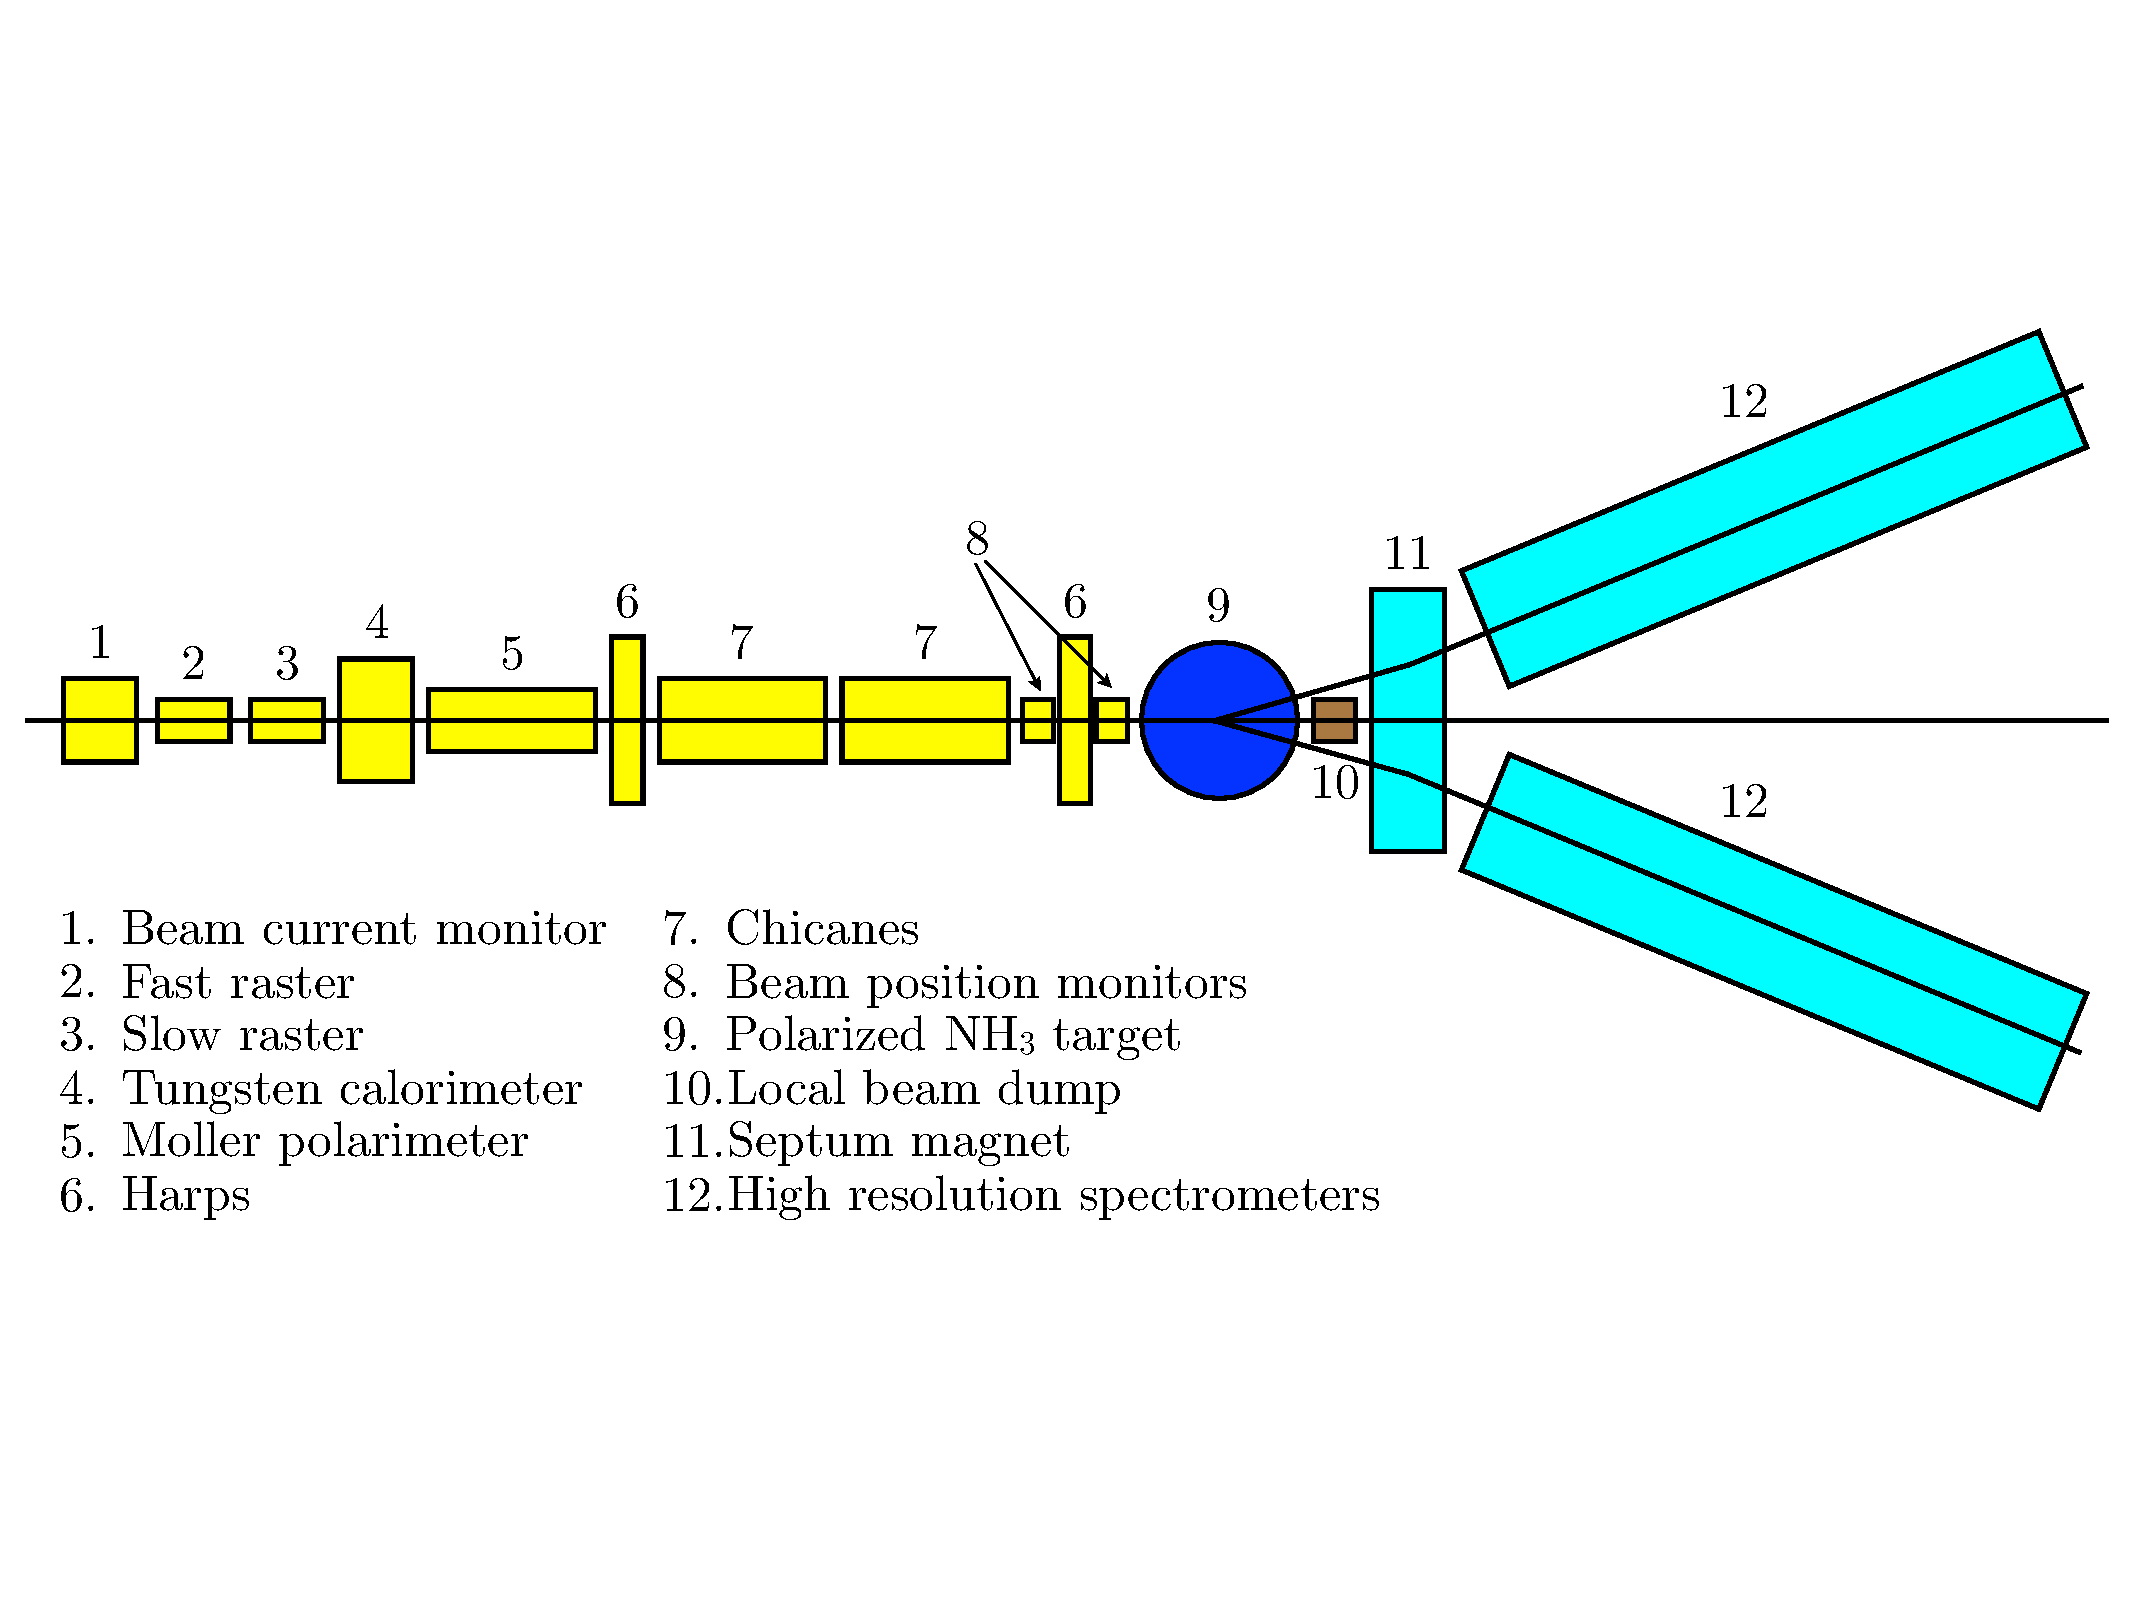
\includegraphics[width=\textwidth]{figs/experiment-setup.pdf}
  \caption[Schematic diagram of the experiment components.]{Schematic diagram of the experiment components. \label{C5S2F1}}
\end{figure}

\subsection{Beam Energy Measurement}
\label{C5S2SS1}

\begin{figure}[b!]
  \centering
  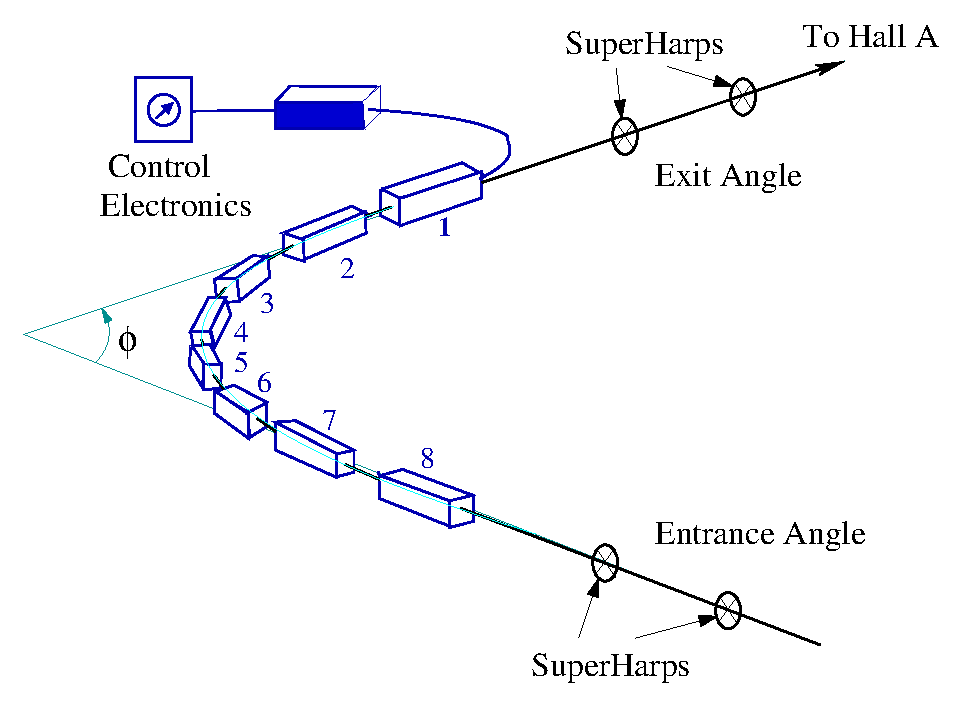
\includegraphics[width=0.75\textwidth]{figs/arc-measurement.pdf}
  \caption[Diagram of the arc section of the beamline.]{Diagram of the arc section of the Hall A beamline. Plot reproduced from \cite{Zheng2002}.  \label{C5S2SS1F1}}
\end{figure}

During E08-027, the beam energy was measured by the Arc method \cite{Alcorn2004}. The idea of the Arc measurement is that the radius of the circular movement of an electron in a magnetic field depends on the field strength and the momentum of the electron. It measures the deflection of the beam in the arc section of the beamline, see \Cref{C5S2SS1F1}. The momentum of the beam $P$ can then be related to the integral of the magnitude of the magnetic field $B$ of the eight dipoles and the net bend angle $\theta$ through the arc sections \cite{BEAMENERGYARC}:
\begin{equation} \label{C5S2SS1E1}
P = k \frac{\int\vec{B}\times\dd{\vec{l}}}{\theta}
\end{equation}
where $k=0.299792$ GeV$\cdot$rad$\cdot$T${}^{-1}\cdot$m${}^{-1}$/c. The Arc method relies on two simultaneous measurements. One is for the actual bend angle of the arc, and the magnetic field integral $\Bdl$ of the eight dipoles in the arc based on a reference magnet measurement. The Arc energy measurement provides an absolute measurement to the $2\times10^{-4}$ GeV level.

\subsection{Beam Current Measurement}
\label{C5S2SS2}

The beam current is measured by two Beam Current Monitors (BCMs). The BCMs used in E08-027 are two stainless steel cylindrical high-$Q$ ($\approx$3000) waveguides (cavities) that are tuned to the frequency of the beam (1497 MHz) \cite{Alcorn2004}. The output voltage signals of the two cavities are proportional to the beam current. The BCM system is composed of two cavities which are located $\approx$23 m upstream from the target center, an Unser monitor and a BCM receiver which converts the raw signals to be compatible with the DAQ system.

Since the standard RMS-to-DC converter of the BCM system \cite{Denard2001} did not work at low beam current, a new BCM receiver designed by the JLab instrumentation group to improve the signal-to-noise (S/N) ratio in an environment with beam current from several nano-ampere to several micro-ampere \cite{Musson2012}. The receiver is composed of an analog part, which converts the radiofrequency (RF) signal from the cavities to the intermediate frequency (IF) signal and amplify it, and a digital part, which provides several digital filters to reduce the S/N ratio.

The RF signal with a frequency $\omega=1497$ MHz (same as beam) is mixed multiplicatively with a sinusoidal $\omega'=1452$ MHz signal from a local oscillator. Thus the mixed signal could be decomposed to a high frequency component with frequency $\omega+\omega'$ and a low frequency component with frequency $\omega-\omega'=45$ MHz. The high frequency signal is filtered out.

The 45 MHz intermediate frequency signal is amplified twice and is digitized by an analog-to-digital convertor (ADC). Two digital filters are applied to the digital signal, which can achieve higher stop-band attenuation, faster transition and higher efficiency. The cut-off frequency of the filter is set to 10.4 kHz for the BCM receiver to achieve enough S/N ratio. After the filter, the digital signal is converted back to a 0$\sim$10 V analog signal to match the input of the existed Hall A DAQ system. A voltage-to-frequency module in the DAQ system converts the voltage signal to the frequency signal and is counted by the scalers.

Usually the BCMs are calibrated with the Faraday cup in the injector. The Unser monitor located between two RF cavities could also be used to give a cross-check of the Faraday cup calibration result. However, both methods can not work at low beam currents. Therefore a tungsten calorimeter \cite{Bevins2005} was installed to calibrate our BCMs with the heating effect of the electron beam.

During the calibration, the beam is incident to the tungsten block in the calorimeter. All the electrons are stopped by the tungsten causing the temperature of the block to increase during the beam. The tungsten block is held in a vacuum chamber to minimize heat loss. The relation between the total charge $Q$ and the increased temperature $\Delta T$ is:
\begin{equation} \label{C5S2SS2E1}
Q = e\cdot\frac{K_{\mathrm{W}}\cdot\Delta T}{E_{\mathrm{Beam}}},
\end{equation}
where $E_{\mathrm{Beam}}$ is the beam energy, and the $K_{\mathrm{W}}$ is the heat capacity of the tungsten. $K_{\mathrm{W}}$ of the tungsten block used in the experiment was measured before the experiment, which is 8555.5$\pm$50 J/K \cite{CTUNGSTEN}.

Once the $Q$ for a calibration run is known, the scaler readout is calibrated via the formula:
\begin{equation} \label{C5S2SS2E2}
N = (C\cdot I+C_0)\cdot t,
\end{equation}
where $N$ is the BCM scaler reading, $C$ is the calibration constant and $C_0$ is the pedestal value of the BCM.

The uncertainty of the calibration could arise from the uncertainty of the beam energy, the temperature and the heat capacity of the tungsten as well as the effect from heat loss. The uncertainty of the beam energy measurement at Hall A is at the $2\times10^{-4}$ level \cite{BEAMENERGY}. The uncertainties of the temperature sensors are 12.5 mK \cite{CALORIMETERLEDEX}. The uncertainty of the tungsten heat capacity is 50 J/K. The Hall A calorimeter thermal and mechanical design assures that the heat loss is at $\approx$0.2\% level if the measurement takes less than 20 minutes \cite{Bevins2005}. Combining all of these effects, one could get the uncertainty of the calibration to be 0.7\% on the beam current.

Since the beam current is measured by two cavities independently, the difference between the upstream and downstream BCM could be used to estimate the uncertainty of the BCM readout. The relative differences between the two BCMs are below 0.7\% for 90\% of the runs. See Ref. \cite{Zhu2015} for detailed discussions of the BCM calibration and the uncertainty estimation.

\subsection{Beam Position Measurement}
\label{C5S2SS3}

Two Beam Position Monitors (BPMs) located 95.5 cm and 69.0 cm upstream from the target center were used to determine the position and direction of the beam at the target center. Each BPM contains four wire antennas parallel to the beam direction, which are placed symmetrically around the beam pipe in a vacuum chamber. When the beam passes through the BPM system, a signal is induced in each antenna. The size of each induced signal is inversely proportional to the distance from that antenna to the beam \cite{Barry1991}. \Cref{C5S2SS3F1} shows the structure of a BPM. With the assumption that the chamber is long enough so that the edge effect could be neglected and the antenna did not influence the electric field inside the chamber, the amplitude of the signal received by each antenna can be expressed as \cite{Piot2005}:
\begin{equation} \label{C5S2SS3E1}
\varphi_i = \varphi_0 I\frac{R^2-\rho^2}{R^2+\rho^2-2R\rho\cos(\theta_i-\theta_0)},
\end{equation}
where $i$ is one of four antennas $u_+$, $u_-$, $v_+$ and $v_-$, $\varphi_0$ is a constant related to the geometry of the BPM chamber and the output resistance, $I$ is the beam current, $R$ is the radius of the BPM chamber, $\rho$ is the radial position of the beam and $\theta_i-\theta_0$ is the angle difference between the antenna and the beam in a polar coordinates.

\begin{figure}[b!]
  \centering
  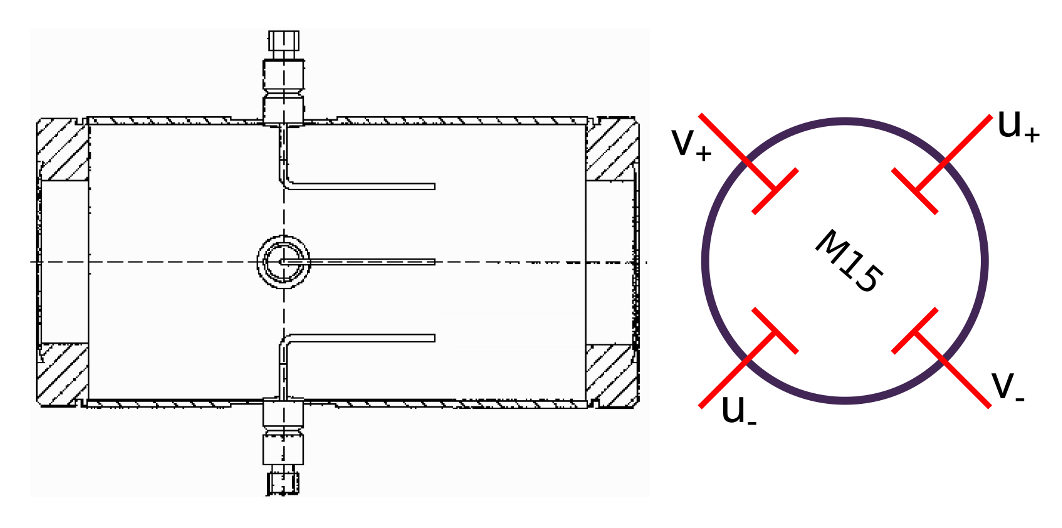
\includegraphics[width=0.7\textwidth]{figs/bpm-design.png}
  \caption[Diagram of the BPM.]{Diagram of the BPM. \label{C5S2SS3F1}}
\end{figure}

The beam position $u$ and $v$ could be extracted in the BPM local coordinates. The $u_+$ and $u_-$ antennas define the $\hat{u}$ axis of this coordinate system and the $v_+$ and $v_-$ antennas define the $\hat{v}$ axis. If $u^2+v^2\ll R^2$, the beam position can be expressed as:
\begin{equation} \label{C5S2SS3E2}
W \approx \frac{R}{2}D_W,
\end{equation}
with
\begin{equation} \label{C5S2SS3E3}
D_W= \frac{R}{2}\frac{\varphi_{W_+}-\varphi_{W_-}}{\varphi_{W_+}+\varphi_{W_-}}.
\end{equation}
Here $W$ denotes $u$ or $v$. Since the beam is circularly rastered with a diameter of 2 cm in E08-027 and the radius of the BPM chamber $R$ is only 1.73 cm, \cref{C5S2SS3E2} is no longer valid, and the beam position must be calculated via a corrected formula:
\begin{equation} \label{C5S2SS3E4}
W = RD_W\left(\frac{1}{D^2}-\frac{1}{D}\sqrt{\frac{1}{D^2}-1}\right),
\end{equation}
with $D^2=D_u^2+D_v^2$.

Like the BCMs, the BPM system also contains a receiver which collects and sends the signal to the DAQ system. As mentioned in \Cref{C5S2SS2}, the original receiver did not work at low beam currents, thus a new BPM receiver was designed by the JLab instrumentation group \cite{Musson2012} to be compatible with beam current as low as 50 nA. The output signal of the receiver is sent to a 13-bit fastbus ADC with an integration time of 50 ns which is triggered by a detected event. The BPM receiver shares the same design with the BCM receiver, but the cut-off frequency of the digital filter of the BPM receiver is set to 175 Hz to increase the S/N ratio and reach the required resolution. This leads to a 1/175 s delay of the beam position signal. There is also a $\approx$4 $\mu$s delay as the processing time of the electronics. Since the beam is spread by a 25 kHz fast raster, the BPM could not provide the beam position event by event due to the time delay effect. Thus the BPM is only used to measure the center of the raster pattern, the raster information is combined with the BPM readout to provide the beam position for each event. The magnet current of the rasters is calibrated to get the absolute values of the deviations with respect to the center of the raster pattern. The details of the rasters used in the experiment will be discussed in \Cref{C5S2SS5}.

\begin{figure}[tb!]
  \centering
  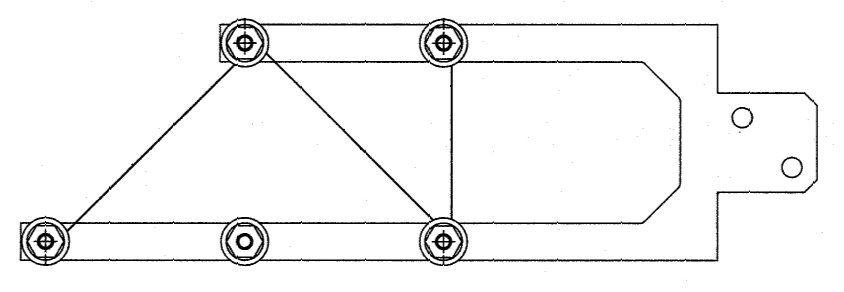
\includegraphics[width=0.5\textwidth]{figs/harp.png}
  \caption[Diagram of the harp.]{Diagram of the harp. \label{C5S2SS3F2}}
\end{figure}

The BPMs are calibrated with two superharps. One harp is installed between the 2 BPMs and the other one is installed upstream of the upstream chicane magnet. \Cref{C5S2SS3F2} shows a schematic diagram of the harp. The harp consists of three wires with a thickness of 50 $\mu$m which are fixed to a chassis controlled by a step motor \cite{Yan1995}. The original position of each wire is surveyed with a precision level of 0.1 mm. During the calibration, the harp is moved into the beam pipe by the step motor. The wires are scanned by the electron beam resulting showers of particles which can be detected. The absolute beam position could be calculated with the recorded wire signal and the survey result. Meanwhile the beam position is also measured with BPMs. By comparing the BPM readout and the harp wire signal, the BPMs can be calibrated.

The BPMs only measure the beam position at their own locations. Usually the beam positions at BPMs could be linearly projected to the target location to retrieve the beam positions at the target. However, the transverse target field in E08-027 breaks the linear projection. A simulation package was constructed to trace the movement of the incident electrons in the target field. The beam trajectories generated by the simulation package are used to fit a set of transport functions which could transport the beam positions at two BPMs to the spatial coordinates and the incident angles of the beam at the target location. These transport functions are used to calculate the beam position at the target location.

The uncertainty of the final beam position at the target location arises from several sources such as the uncertainty of the harp calibration constant, the survey data and the pedestal value of the electronics. The final uncertainty of the beam position is 1$\sim$2 mm, while the uncertainty of the incident angle is 1$\sim$2 mrad. See Ref. \cite{Zhu2014} for detailed discussion of the BPM calibration and the uncertainty estimation.

\subsection{Beam Polarization}
\label{C5S2SS4}

The polarization of the electron beam was measured by the M{\o}ller polarimeter \cite{MOLLER,Alcorn2004} during E08-027. The polarimeter uses polarized M{\o}ller scattering, in which polarized electron beam scatters off polarized atomic electrons in a magnetized ferromagnetic foil $\vec{e}\,^-+\vec{e}\,^-\rightarrow e^-+e^-$, to measure the beam polarization. \Cref{C5S2SS4F1} shows a sketch of the M{\o}ller polarimeter. The polarimeter is composed of three quadrupoles and a dipole. The detector system consists of scintillators and lead-glass calorimeter modules.

\begin{figure}[b!]
  \centering
  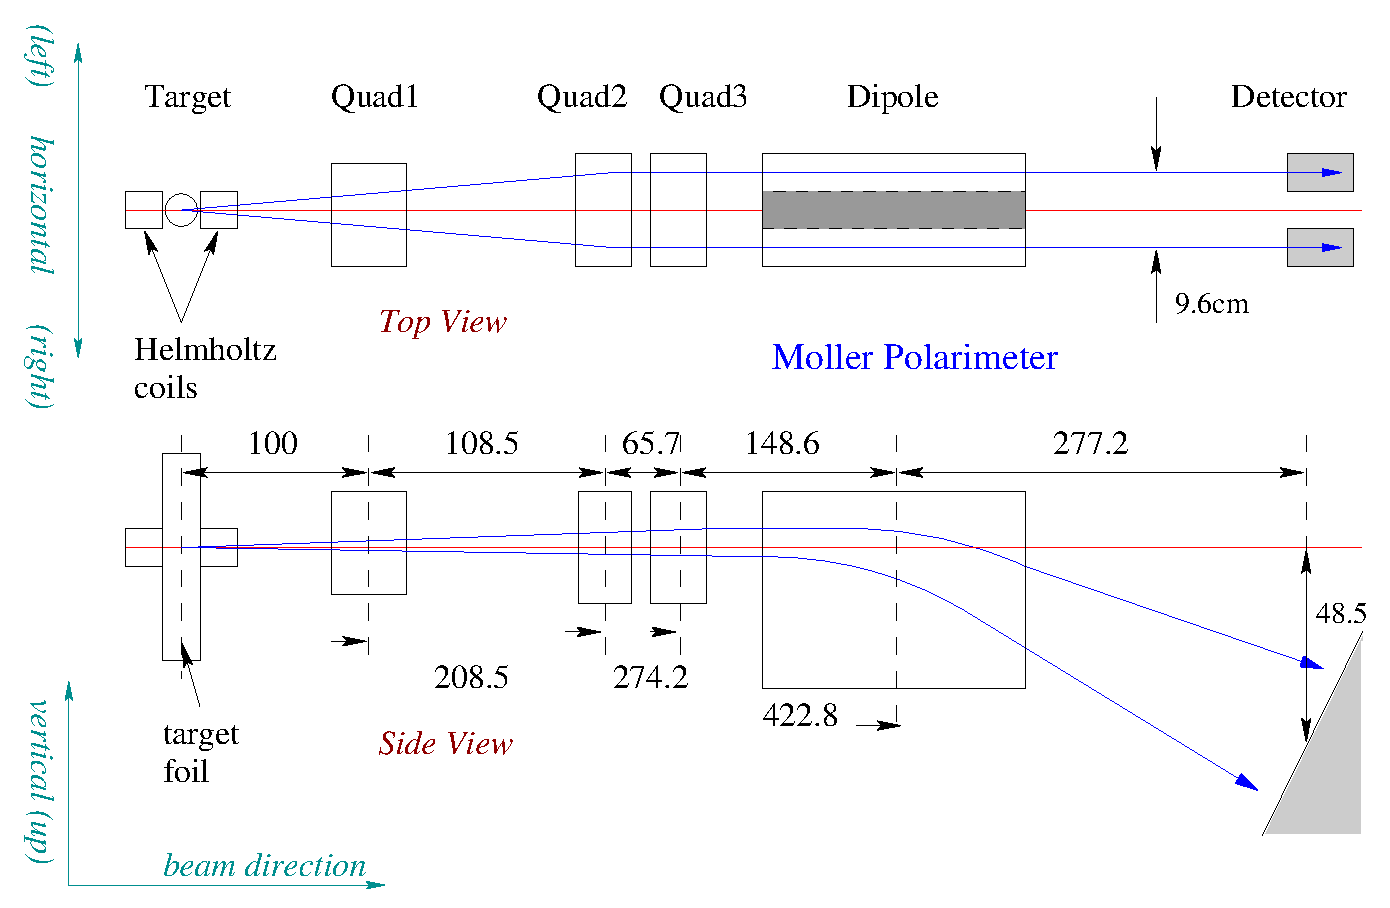
\includegraphics[width=\textwidth]{figs/moller.pdf}
  \caption[Schematic diagram of the M{\o}ller polarimeter.]{Schematic diagram of the M{\o}ller polarimeter. Plot reproduced from \cite{Zheng2002}. \label{C5S2SS4F1}}
\end{figure}

The M{\o}ller scattering cross-section can be expressed in terms of the beam polarization $P_{\mathrm{beam}}^i$ and target polarization $P_{\mathrm{target}}^i$ \cite{Alcorn2004}:
\begin{equation} \label{C5S2SS4E1}
\sigma = \sigma_0\left[1+\sum_{i=x,y,z}A_{ii}P_{\mathrm{beam}}^iP_{\mathrm{target}}^i\right],
\end{equation}
where $i$ is the projection direction of the polarization, and $\sigma_0$ is the unpolarized M{\o}ller cross-section. The coordinate system is defined such that the beam direction is along the $z$-axis and the $y$-axis is perpendicular to the scattering plane. The $A_{ii}$ are the analyzing powers which can be expressed as:
\begin{align} \label{C5S2SS4E2}
A_{zz} & = -\frac{\sin^2\theta_{\mathrm{cm}}\cdot(7+\cos^2\theta_{\mathrm{cm}})}{(3+\cos^2\theta_{\mathrm{cm}})^2}, \\ \label{C5S2SS4E3}
A_{xx} & = -A_{yy} =  -\frac{\sin^4\theta_{\mathrm{cm}}}{(3+\cos^2\theta_{\mathrm{cm}})^2},
\end{align}
where $\theta_{\mathrm{cm}}$ is the scattering angle in the center-of-mass frame. Since the beam is longitudinally polarized, the corresponding analyzing power is $A_{zz}$, which reaches its maximum value of $7/9$ when $\theta_{\mathrm{cm}}=$\SI{90}{\degree}. The polarized M{\o}ller cross-sections are less sensitive to the transverse polarization and the data with opposite target transverse polarization could be averaged to cancel the transverse contributions.

During the experiment, a pair of asymmetries are measured at two target angles of about $\pm$\SI{20}{\degree} with respect to the beam in the horizontal plane, and the average is taken to cancel the transverse contributions as mentioned above. Here asymmetries are measured rather than cross-sections since the asymmetry is a ratio of cross-sections, thus most of the systematic uncertainties related to the cross-section measurement cancel out when taking the ratio.

The beam longitudinal polarization is measured as:
\begin{equation} \label{C5S2SS4E4}
P_{\mathrm{beam}} = \frac{1}{P_{\mathrm{target}}\cos\theta_{\mathrm{target}}\expval{A_{zz}}}\times\frac{N_+-N_-}{N_+-N_-},
\end{equation}
where $N_+$ and $N_-$ are the detected events with opposite orientations of beam polarization. The average analyzing power $\expval{A_{zz}}$ is  calculated with a Monte-Carlo simultion of the M{\o}ller polarimeter. Nine measurements were taken during the experiment, which were scheduled during beam unavailable periods or during a configuration change in the accelerator. The M{\o}ller measurement results are shown in \cref{C5S2SS4T1}. The statistical accuracy is typically 0.2\% as discussed in Ref. \cite{Alcorn2004}. There is a $\approx$1.7\% relative systematic uncertainty dominated by the knowledge of the foil polarization \cite{MOLLER}.

\begin{table}[tb!]
  \centering
  \newcolumntype{C}[1]{>{\centering\arraybackslash}m{#1}}
  \begin{tabular}{|c|c|C{3.5cm}|C{2.5cm}|}
    \hline
      & Date & Polarization and Statistical Error (\%) & Systematic Error (\%) \\ \hline
    1 & 03/03/2012 & 79.91$\pm$0.20 & $\pm$1.7 \\ \hline
    2 & 03/30/2012 & 80.43$\pm$0.46 & $\pm$1.7 \\ \hline
    3 & 03/30/2012 & 79.89$\pm$0.58 & $\pm$1.7 \\ \hline
    4 & 04/10/2012 & 88.52$\pm$0.30 & $\pm$1.7 \\ \hline
    5 & 04/23/2012 & 89.72$\pm$0.29 & $\pm$1.7 \\ \hline
    6 & 05/04/2012 & 83.47$\pm$0.57 & $\pm$1.7 \\ \hline
    7 & 05/04/2012 & 81.82$\pm$0.59 & $\pm$1.7 \\ \hline
    8 & 05/04/2012 & 80.40$\pm$0.45 & $\pm$1.7 \\ \hline
    9 & 05/15/2012 & 83.59$\pm$0.31 & $\pm$1.7 \\ \hline
  \end{tabular}
  \caption[Beam energy and target field configurations.]{Summary of the M{\o}ller measurement result. Table reproduced from \cite{MOLLERG2P}. \label{C5S2SS4T1}}
\end{table}

\subsection{New Instruments}
\label{C5S2SS5}

\subsubsection{Raster System}

The target used in E08-027 is a polarized NH${}_3$ target, which will be described in \Cref{C5S3}. It was operated at $\approx$1 K and would depolarize if the target material was heated by the electron beam. Thus the beam position must be moved constantly to avoid localized overheating of the target material. A uniform distribution of beam on the target was achieved by moving the beam position with time-varying dipole magnetic fields. These dipoles were referred to as rasters.

Two raster systems, the fast raster and the slow raster, were installed at $\approx$17 m upstream from the target center. The fast raster is a standard Hall A beamline component, which consists of two dipole magnets. Both of the dipoles were driven by the same current in a triangular waveform with a frequency of 25 kHz. The beam position was moved by the dipole fields in $\hat{x}$ and $\hat{y}$ directions, respectively, and formed a 2 mm $\times$ 2 mm rectangular pattern. The shape of the fast raster pattern is shown in \Cref{C5S2SS5F1}.

\begin{figure}[tb!]
  \centering
  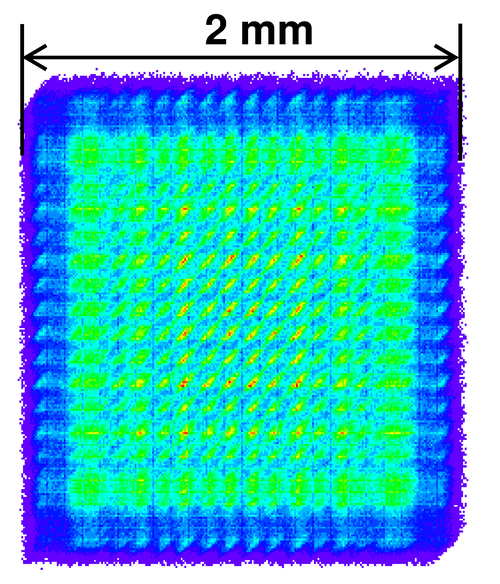
\includegraphics[width=0.2\textwidth]{figs/fast-raster-pattern.png}
  \caption[Fast raster pattern.]{Fast raster pattern. The plot is produced from the magnet current signal. \label{C5S2SS5F1}}
\end{figure}

The target cell of E08-027 is a cylinder with $\approx$25 mm diameter. Thus the fast raster is not enough to spread the beam uniformly on to the whole target. A slow raster was installed in Hall A immediately downstream of the fast raster. The slow raster also consists of two dipole magnets, however the drive current of the dipoles is not in triangular waveform. The waveform used in the slow raster was generated from a dual-channel function-generator:
\begin{align} \label{C5S2SS5E1}
I_x & = I_x^{\mathrm{max}}f(t^{\frac{1}{2}})\sin(\omega t), \\ \label{C5S2SS5E2}
I_y & = I_y^{\mathrm{max}}f([t+t_0]^{\frac{1}{2}})\cos(\omega t),
\end{align}
for the $\hat{x}$ and $\hat{y}$ directions, respectively. Here the $I_x^{\mathrm{max}}$ and $I_y^{\mathrm{max}}$ are the maximum amplitude. \cref{C5S2SS5E1,C5S2SS5E2} are parametric equations of a circle which is modulated by a function $f(t^{\frac{1}{2}})$ to generate a uniform circular pattern \cite{Yan2005}, up to $\approx$20 mm diameter for E08-027. The amplitude modulation (AM) function $f(t^{\frac{1}{2}})$ is a periodic piecewise function with frequency $1/T$, which can be expressed as (in the first period):
\begin{equation} \label{C5S2SS5E3}
f(t) =
\begin{cases}
t^{\frac{1}{2}}, & \text{if } 0\leq t<T/4, \\
(T/2-t)^{\frac{1}{2}}, & \text{if } T/4\leq t<T/2, \\
-(t-T/2)^{\frac{1}{2}}, & \text{if } T/2\leq t<3T/4, \\
-(T-t)^{\frac{1}{2}}, & \text{if } 3T/4\leq t<T.
\end{cases}
\end{equation}
The $t_0$ in \cref{C5S2SS5E2} is the phase difference between the AM functions in the $\hat{x}$ and $\hat{y}$ directions. \Cref{C5S2SS5F2} indicates the effect of $t_0$.

\begin{figure}[tb!]
  \centering
  \begin{subfigure}[t]{0.25\textwidth}
    \centering
    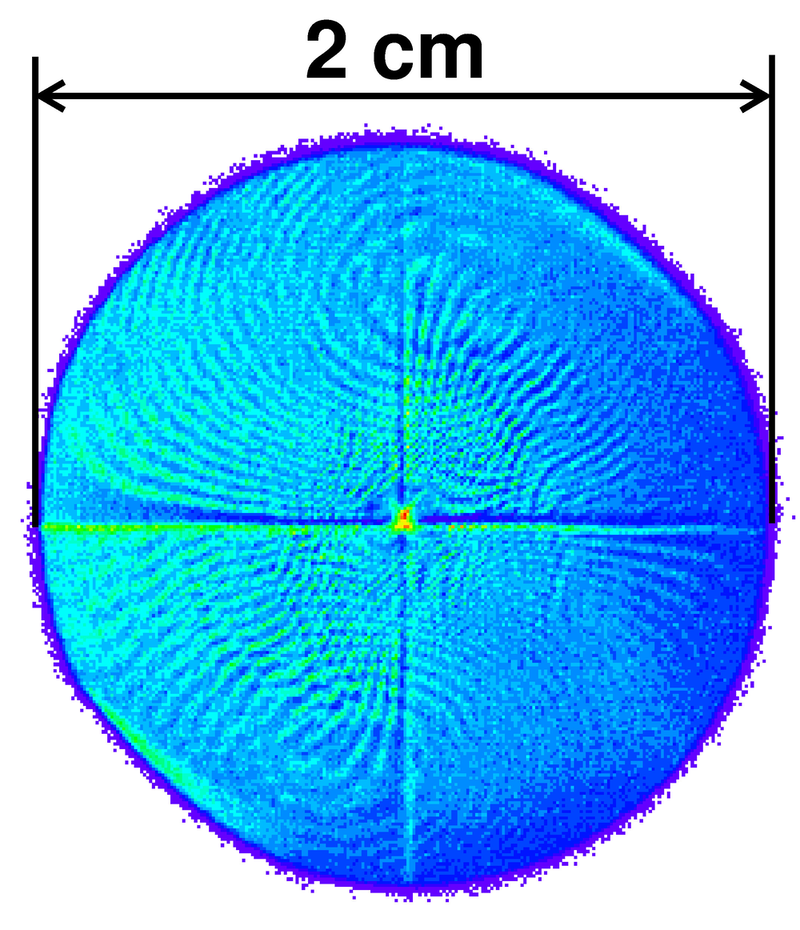
\includegraphics[width=0.8\textwidth]{figs/slow-raster-pattern.png}
    \caption{Slow raster magnet current distribution. \label{C5S2SS5F2a}}
  \end{subfigure}
  \qquad
  \begin{subfigure}[t]{0.25\textwidth}
    \centering
    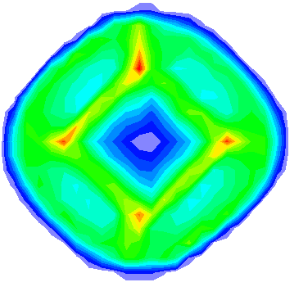
\includegraphics[width=0.8\textwidth]{figs/slow-raster-pattern-data-bad.png}
    \caption{Slow raster pattern with $t_0\neq0$. \label{C5S2SS5F2b}}
  \end{subfigure}
  \qquad
  \begin{subfigure}[t]{0.25\textwidth}
    \centering
    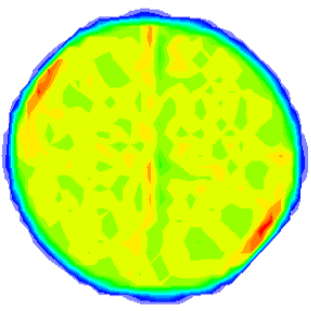
\includegraphics[width=0.8\textwidth]{figs/slow-raster-pattern-data-good.png}
    \caption{Slow raster pattern with $t_0=0$. \label{C5S2SS5F2c}}
  \end{subfigure}
  \caption[Slow raster pattern.]{Slow raster pattern. Here (a) is produced from the magnet current distribution, (b) and (c) are produced from the BPM readout of the slow raster pattern with different $t_0$ settings. \label{C5S2SS5F2}}
\end{figure}

During E08-027, the frequency $\omega$ in \cref{C5S2SS5E1,C5S2SS5E2} was 99.412 Hz. The frequency $1/T$ of the AM function was set to 30 Hz. The phase difference $t_0$ was manually adjusted to be 0. As shown in \Cref {C5S2SS5F2b}, a non-zero $t_0$ could cause a non-uniform pattern. Thus, $t_0$ was carefully minimized during the experiment to avoid the non-uniformity. The pattern of the beam was relatively uniform after the adjustment as shown in \Cref{C5S2SS5F2c}.

\subsubsection{Chicane Magnets}

The strong transverse magnetic field in the target region influences the electron beam. The direction of the magnetic field was pointing to the left of the beam if looking along the downstream direction. According to the right-hand rule, the electron beam would be deflected downwards in the target field. Two chicane magnets were placed in front of the target and the BPMs to provide an upward incident angle for the electron beam when it reaches the center of the target. \Cref{C5S2SS5F3} shows the effects of the chicane magnets and the target field on the electron beam. The first chicane magnet, installed 5.92 m upstream from the target center, bent the beam downwards. The second chicane magnet, installed 2.66 m upstream from the target center, bent the beam back towards the target but at an angle to compensate for further bending from the target field. The vertical position of the chicane magnets was adjusted according to the beam energy and the target field configuration during the experiment such that when the beam hit the target, its direction is parallel to the beamline.

\begin{figure}[tb!]
  \centering
  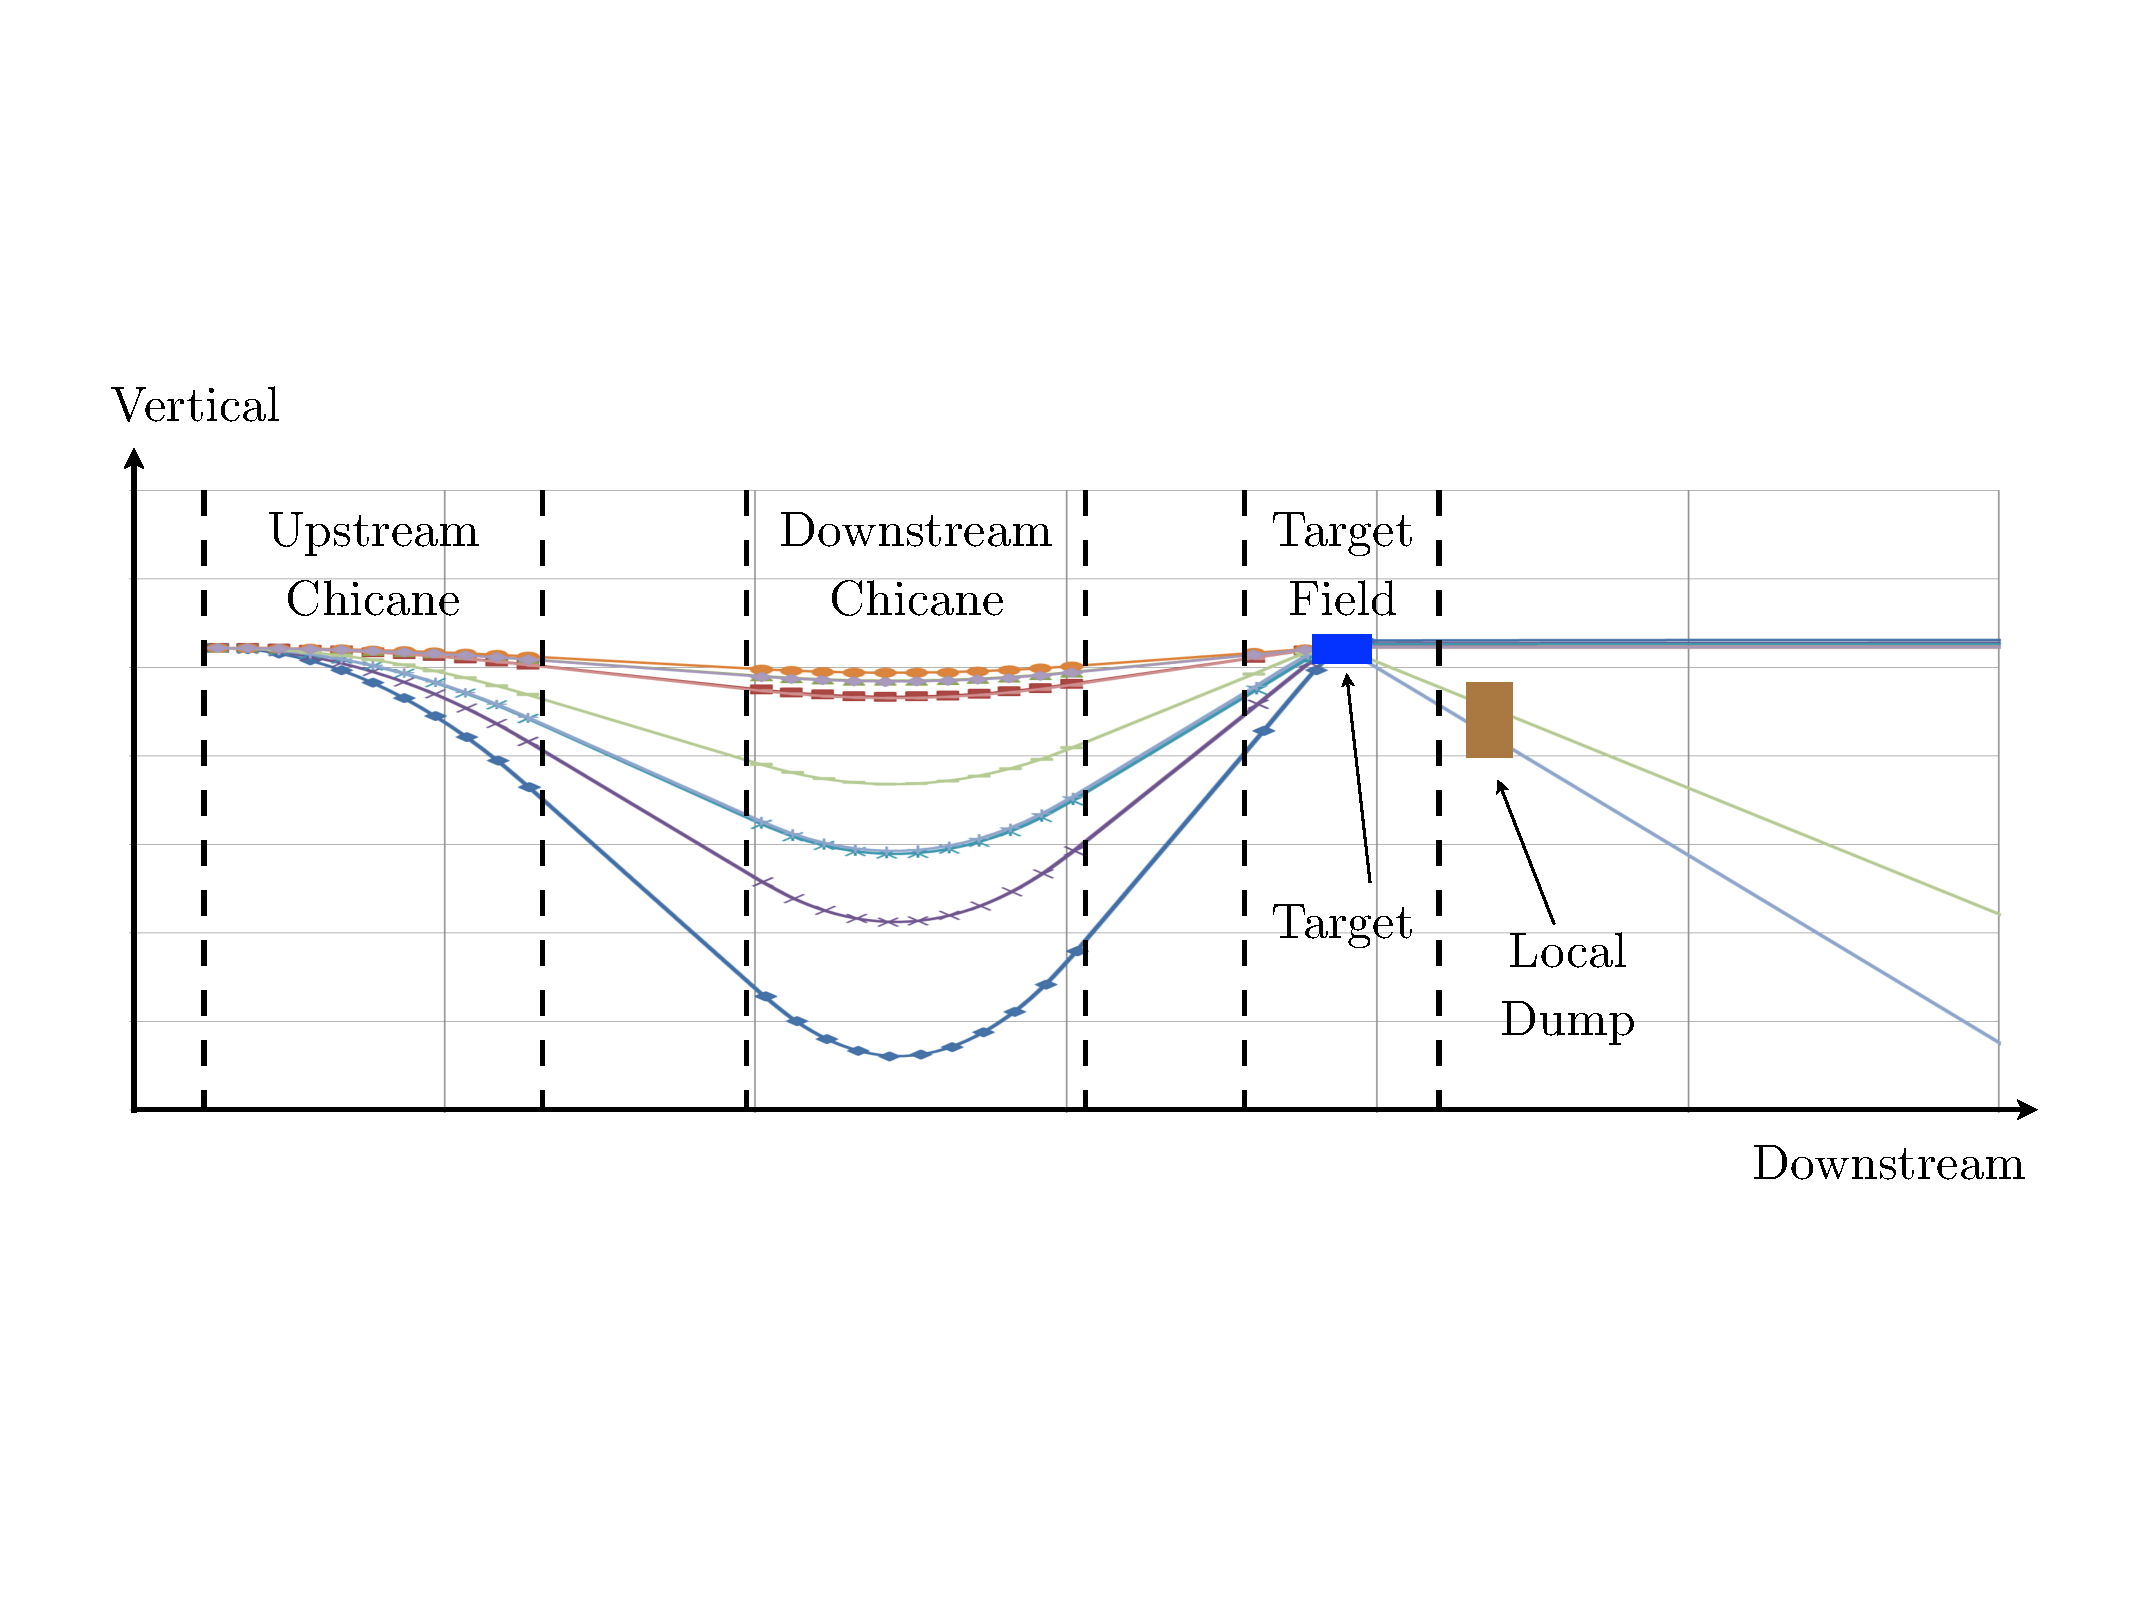
\includegraphics[width=0.9\textwidth]{figs/beam-traj.pdf}
  \caption[Schematic diagram of the effects of the chicane magnets.]{Schematic diagram of the effects of the chicane magnets and the target field on the electron beam. The trajectories are marked with different colors for different beam energy and target field configuration. Notice the diagram does not reflect the actual scale of each component. \label{C5S2SS5F3}}
\end{figure}

\subsubsection{Local Beam Dump}

As seen in \Cref{C5S2SS5F3}, most of the beam trajectories exit the target field region horizontally (in these cases the target field strength is 2.5 T), and could reach the Hall A beam dump. However, the chicane magnets could not bend the beam to the Hall A beam dump for those configurations with the 5.0 T transverse target field due to the limited installation space for the chicane magnets. Since the beam current was quite low for this experiment, a local beam dump which consisted of a series of tungsten and copper plates was used to stop the beam which could not reach the Hall A beam dump. The local beam dump was installed 0.64 m downstream of the center of the polarized target as shown in \Cref{C5S2SS5F3}. The local beam dump worked well during the experiment and successfully protected the electronics in the experimental hall from high radiation background.

\section{\texorpdfstring{Polarized NH${}_3$ Target}{Polarized NH3 Target}}
\label{C5S3}

In E08-027, a polarized ammonia NH${}_3$ target was used to provide the polarized proton target. Since the nucleons in the nitrogen nuclei are not coupled with the electrons, they would not be polarized by the Dynamic Nuclear Polarization (DNP) method. This target has been successfully used for several JLab experiments prior to E08-027. The target has demonstrated a high proton polarization up to 90\% with a 5.0 T target field. The 5.0 T target field was used in E08-027 and a new 2.5 T configuration was operated in this experiment for the first time.

\subsection{Dynamic Nuclear Polarization}
\label{C5S3SS1}

The DNP method is used to polarize the hydrogen nuclei in a NH${}_3$ target. Zeeman effect tells us that a spin non-zero particle located in a strong magnetic field is polarized spontaneously. If the magnetic moment of the particle is $\mu$ and the spin is 1/2, the ground state of this particle splits to two sublevels with energy $E_0+\mu B$ and $E_0-\mu B$, respectively. The population of these two sublevels follows Maxwell-Boltzmann statistics:
\begin{equation} \label{C5S3SS1E1}
N(E_0\pm\mu B) = N(E_0)\exp(-\frac{\pm\mu B}{k_B T}),
\end{equation}
where $k_B$ is the Boltzmann constant and $T$ is the temperature of the system. Thus the spontaneous polarization of the material is:
\begin{equation} \label{C5S3SS1E2}
P_{\mathrm{TE}} = \frac{\exp(\frac{\mu B}{k_BT})-\exp(-\frac{\mu B}{k_BT})}{\exp(\frac{\mu B}{k_BT})+\exp(-\frac{\mu B}{k_BT})} = \tanh(\frac{\mu B}{k_B T}).
\end{equation}
where TE stands for thermal equilibrium and we refer to this polarization as the thermal polarization. The magnetic moment of the electron is approximately $\mu_{\mathrm{B}}\equiv e\hbar/2m_e$ and the magnetic moment of the proton is only $1.521\times10^{-3}\mu_{\mathrm{B}}$ due to the mass difference. From \cref{C5S3SS1E2}, we know that the thermal polarization of a sample of electrons is above 90\% but the proton's thermal polarization is only $\approx$2.5\% for the 1 K temperature and 2.5 T magnetic field, the typical target configuration in E08-027.

\begin{figure}[tb!]
  \centering
  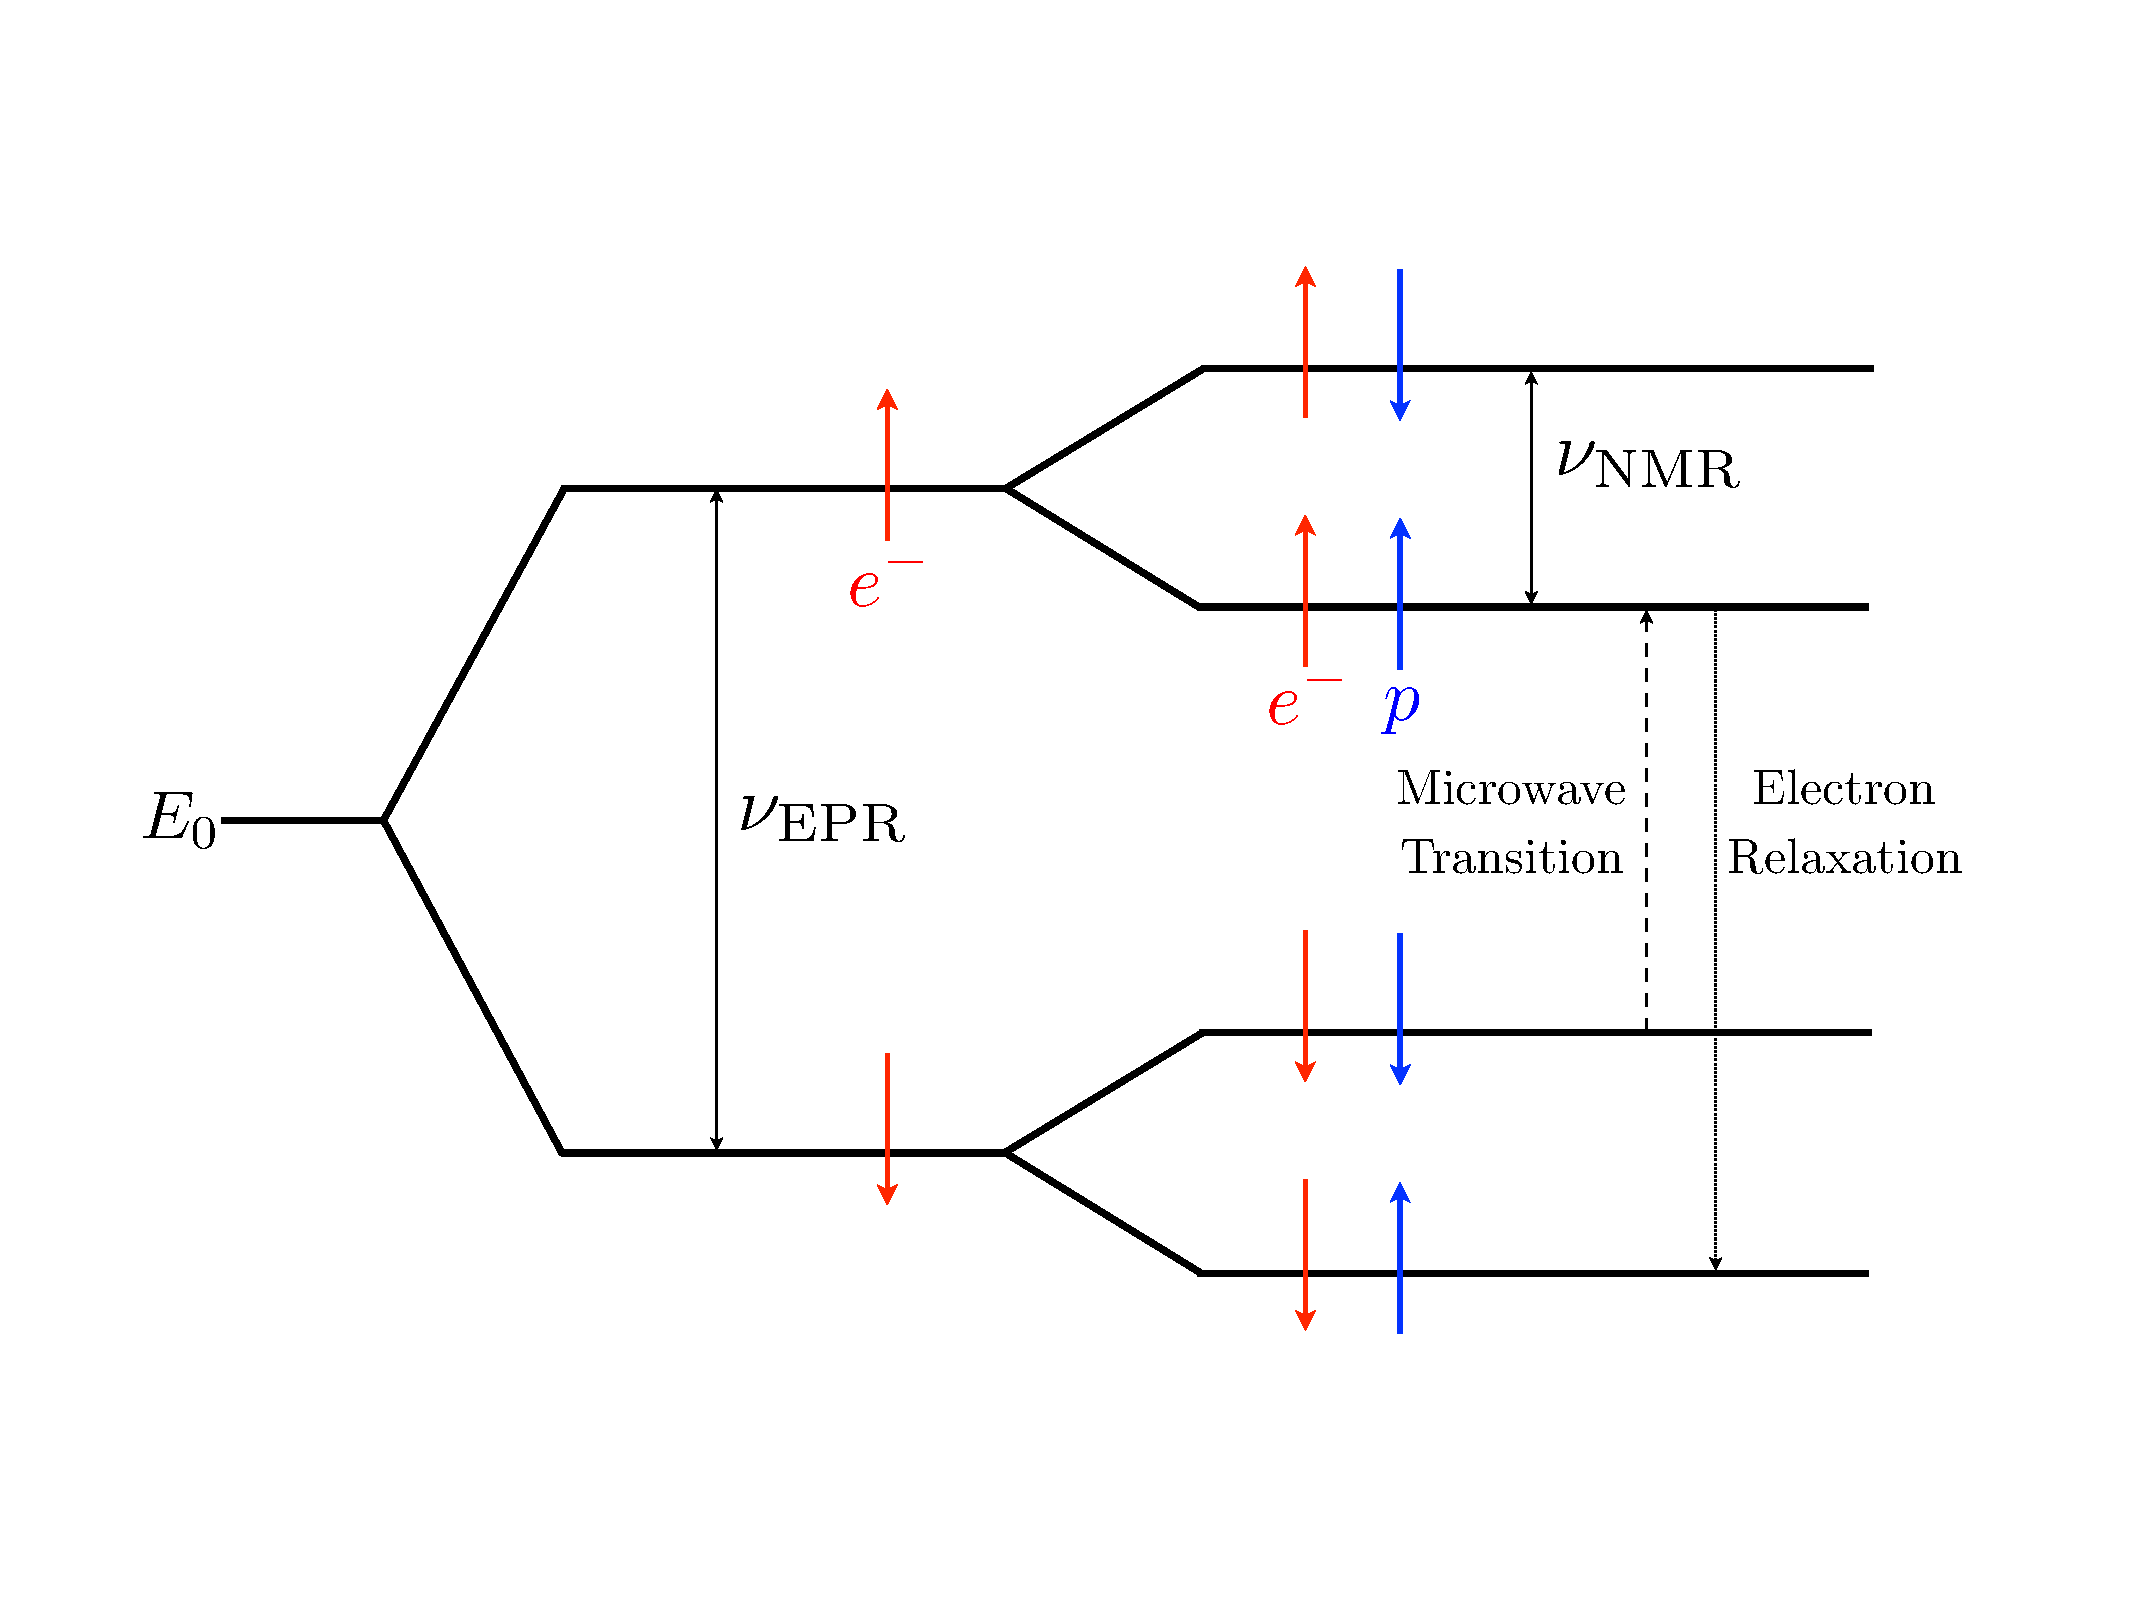
\includegraphics[width=0.6\textwidth]{figs/DNP.pdf}
  \caption[Electron-proton spin coupling interaction diagram.]{Electron-proton spin coupling interaction diagram. \label{C5S3SS1F1}}
\end{figure}

The thermal polarization of the proton is not enough for carring out spin-structure experiments. Thus the DNP method is developed to enhance the polarization by transferring the electron polarization to the nucleon via the electron-proton spin coupling \cite{Overhauser1953,Jeffries1957}. The Hamiltonian of this system can be written as:
\begin{equation} \label{C5S3SS1E3}
H = \vec{\mu_e}\cdot\vec{B}+\vec{\mu_p}\cdot\vec{B}+H_{\mathrm{ss}},
\end{equation}
where $\mu_e$ and $\mu_p$ are the magnetic moments of the electron and proton, respectively, and the $H_{ss}$ arises from the interaction between the electron and proton. The ground state of this system split to four sublevels as shown in \Cref{C5S3SS1F1}, corresponding to the four spin combinations of the electron and the proton. A microwave generator can be used to flip the proton spin and electron spin together if the frequency is carefully tuned at $\nu_{\mathrm{EPR}}-\nu_{\mathrm{NMR}}$ to polarize the proton parallel to the field direction (or $\nu_{\mathrm{EPR}}+\nu_{\mathrm{NMR}}$ for an opposite direction). Here the $\nu_{\mathrm{EPR}}$ is the electron paramagnetic resonance (EPR) frequency and $\nu_{\mathrm{NMR}}$ is the proton nuclear magnetic resonance (NMR) frequency. Since the relaxation time of electrons is only a few milliseconds, the polarized electron is relaxed to the lowest ground state and can be used to polarize a new proton. The relaxation time of protons is tens of minutes so the polarization of protons could be kept if we pump the microwave continuously.

\subsection{Target Setup}
\label{C5S3SS2}

\begin{figure}[b!]
  \centering
  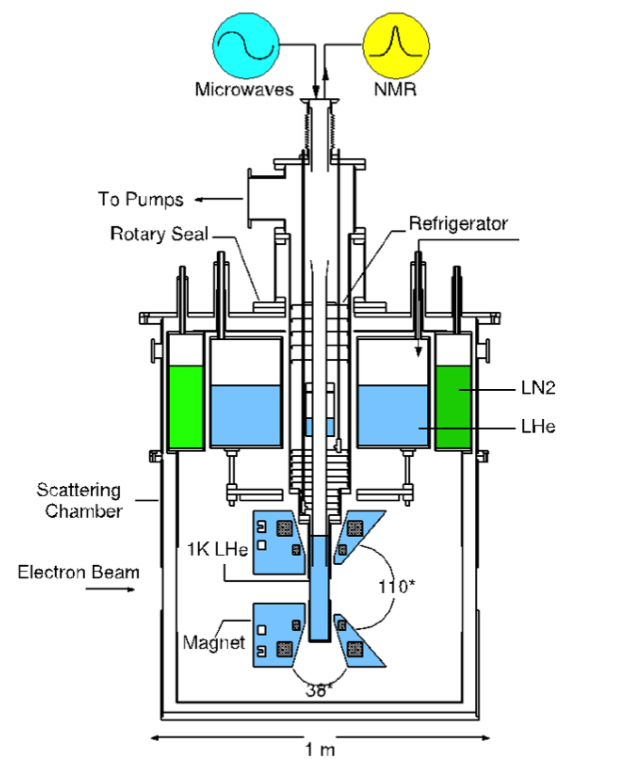
\includegraphics[width=0.6\textwidth]{figs/target.png}
  \caption[Diagram of the polarized NH${}_3$ target system.]{Diagram of the polarized NH${}_3$ target system. \label{C5S3SS2F1}}
\end{figure}

The NH${}_3$ target system used in E08-027 is shown in \Cref{C5S3SS2F1}. The original 5 T Oxford superconducting magnet was burned before the experimentand could not be used. Fortunately, an alternate magnet from Hall B was identified as a suitable replacement. Because of the power and construction limit of the chicane magnets, a 2.5 T field configuration was used in addition to the original 5.0 T magnetic field to reach the minimum possible $Q^2$ with this magnet. The magnetic field must be uniform in order for the DNP process to be efficient. The nonuniformity of the field is less than $10^{-4}$ over the volume of the material which is a cylinder with $\approx$2 cm diameter and $\approx$2 cm length \cite{Pierce2014}. The open geometry of the magnet allows the beam to pass through in both longitudinal and transverse configurations. The magnet is superconducting and is maintained at 4 K with a reservoir of liquid helium.

The target stick can be seen in \Cref{C5S3SS2F2}. The stick contains two NH${}_3$ cells, a carbon foil cell, a ``dummy'' cell and two small disk targets made with carbon and polyethylene respectively. The NH${}_3$ cells are filled with solid NH${}_3$ beads and are covered with aluminum foils. A short Cu-Ni capillary coil is installed in the cell for NMR measurement. The dummy cell is identical to the NH${}_3$ cells which also includes aluminum foils and the NMR coil, but does not contain any NH${}_3$ beads. During the experiment, the end of the target stick is immersed in a container full of liquid helium, which is refered as the target ``nose''. A ${}^4$He evaporation refrigerator was used to cool down the target and maintain its temperature at 1.1 K with 3 W microwave power \cite{Pierce2014}.

\begin{figure}[tb!]
  \centering
  \setlength{\unitlength}{0.1\textwidth}
  \begin{picture}(6.0,2.5)
    \put(0,0){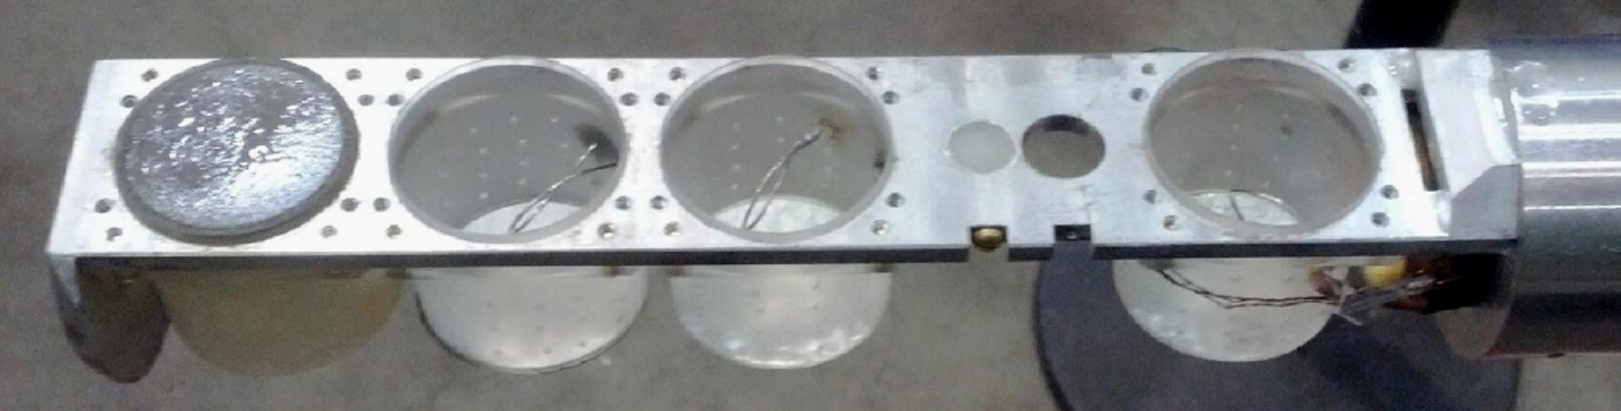
\includegraphics[width=0.6\textwidth]{figs/target-insert.png}}
    \put(0.8,2.0){\makebox(0.1,0.1){Carbon}}
    \put(0.9,1.8){\vector(0,-1){0.5}}
    \put(1.9,1.975){\makebox(0.1,0.1){Dummy}}
    \put(1.9,1.8){\vector(0,-1){0.5}}
    \put(2.8,1.975){\makebox(0.1,0.1){NH${}_3$}}
    \put(2.85,1.8){\vector(0,-1){0.5}}
    \put(4.6,1.975){\makebox(0.1,0.1){NH${}_3$}}
    \put(4.65,1.8){\vector(0,-1){0.5}}
  \end{picture}
  \caption[The end of the target insert.]{The end of the target insert. A carbon foil cell, a ``dummy'' cell and two NH${}_3$ cells are installed in the stick from left to right. And a carbon disk and a polyethylene disk are installed in the holes between two NH${}_3$ cells. \label{C5S3SS2F2}}
\end{figure}

The selection of NH${}_3$ as the target material is due to several reasons. It has been proved that NH${}_3$ is capable of reaching 90\% polarization in a 5 T magnetic field. And it can be polarized within 30 minutes or less, which is very fast compare to other materials. Solid NH${}_3$ also holds up very well against radiation damage which could reduce the polarization rapidly. The radiation can produce additional radicals that reduce the relaxation time of the proton.

\begin{figure}[tb!]
  \centering
  \begin{subfigure}[t]{0.2\textwidth}
    
\includegraphics[width=\textwidth]{figs/ammonia-unirradiated.jpg}
    \caption{Unirradiated. \label{C5S3SS2F3a}}
  \end{subfigure}
  \qquad
  \begin{subfigure}[t]{0.2\textwidth}
    
\includegraphics[width=\textwidth]{figs/ammonia-irradiated.jpg}
    \caption{Irradiated. \label{C5S3SS2F3b}}
  \end{subfigure}
  \caption[NH${}_3$ beads before and after irradiation.]{NH${}_3$ beads before and after irradiation. \label{C5S3SS2F3}}
\end{figure}

On the other hand, radicals in the target material can also allow the material to polarize faster. The NH${}_3$ beads are irradiated with a 10 MeV linear accelerator at the National Institute of Standards and Technology (NIST) before the experiment in order to produce a few additional radicals in the material. The irradiation causes the solid NH${}_3$ beads to become a deep purple color, as seen in \Cref{C5S3SS2F3}. The number of radicals in the material must be carefully balanced: they can speed up the DNP process, but they also increase the speed of the proton depolarization. The DNP process becomes inefficient when the target is exposed in the electron beam long enough with the amount of radicals exceeding the tolerance. To counteract this effect, the target material can be heated up to force the radicals to recombine, which is referred to as the ``annealing'' of the target. During E08-027, the beam current was limited to 50 nA, and the target was annealed periodically. However, there is a limit to how many times the material can be annealed, thus the NH${}_3$ beads still need to be replaced several times during the experiment.

Microwaves are necessary to drive the spin transitions. The microwave generator contains an Extended Interaction Oscillator (EIO) tube to generate the microwave. The microwaves are then carried via waveguides to a horn close to the target cell. The optimal frequency of the microwave radiation is not a constant value due to the radiation damage, thus the frequency need to be tweaked throughout the experiment.

\subsection{Target Polarization Measurement}
\label{C5S3SS3}

The polarization is measured via the NMR method. An LCR circuit with resonance frequency equal to the Larmor frequency of the proton is used as the NMR circuit \cite{Crabb1997}. The power lost or gained in the circuit can be measured via the quality factor ($Q$-factor) of the circuit by a $Q$-meter. The response of the target material to a radiofrequency irradiation is described by its magnetic susceptibility $\chi(\omega)=\chi'(\omega)-i\chi''(\omega)$, where $\chi'(\omega)$ and $\chi''(\omega)$ are the dispersive and absorptive part of the susceptibility respectively. The polarization $P$ of the target is related to the absorptive part of the susceptibility $\chi(\omega)$ \cite{Goldman1975}:
\begin{equation} \label{C5S3SS3E1}
P = K\int_0^\infty\chi''(\omega)\dd{\omega},
\end{equation}
where $K$ is a constant containing the properties of the NMR system. The NMR circuit has inductance $L_C$ and resistance $r_C$ itself, and the inductive coupling between the material and the coil changes the impedance of the circuit to:
\begin{equation} \label{C5S3SS3E2}
Z_C = r_C+i\omega L_C(1+4\pi\eta\chi(\omega)),
\end{equation}
where $\eta$ is the filling factor of the coil. The circuit is driven by an RF generator which sweeps through a range of frequencies around the Larmor resonance of the circuit.

\begin{figure}[p!]
  \centering
  \begin{subfigure}[t]{0.49\textwidth}
    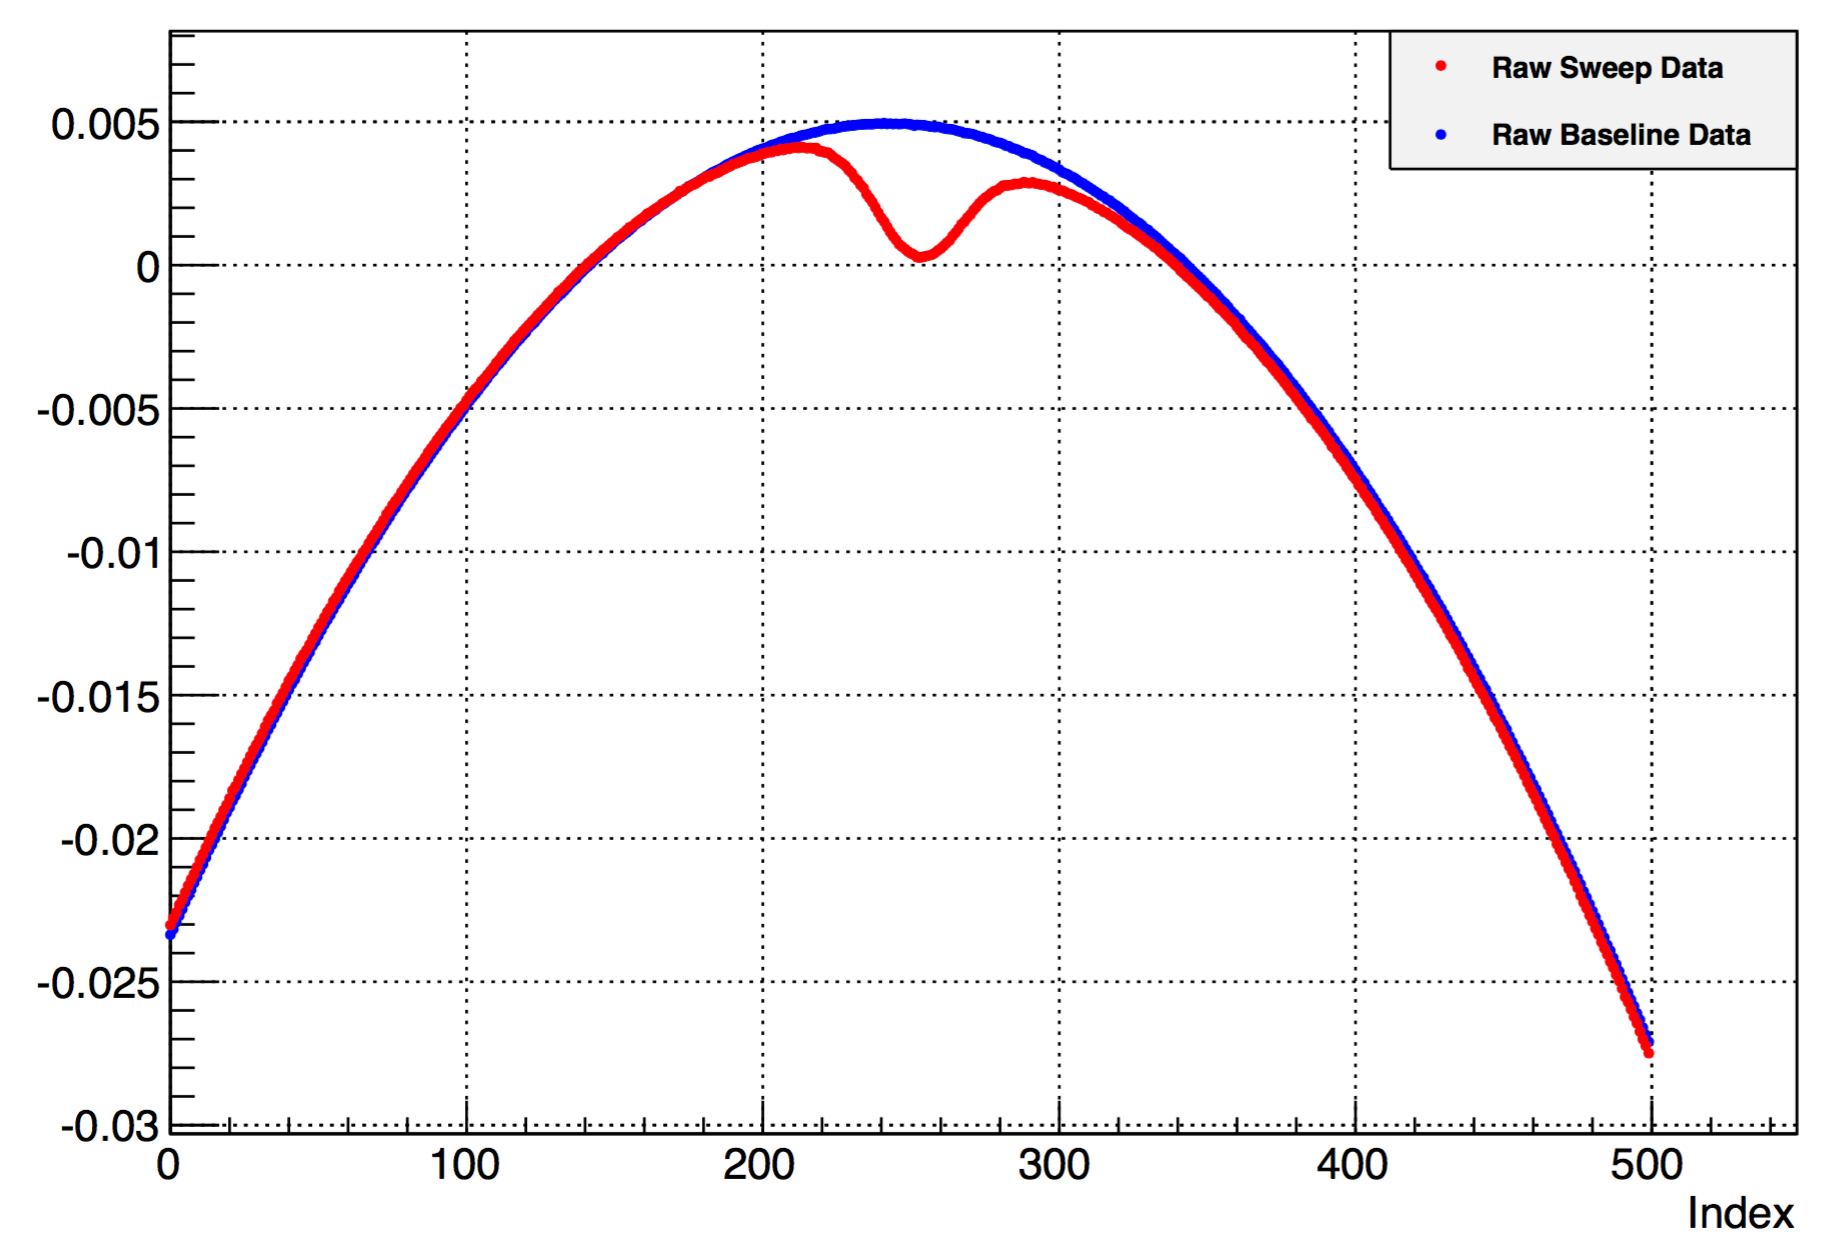
\includegraphics[width=\textwidth]{figs/target-NMR-raw.png}
    \caption{The raw signal (red) and the baseline signal ($Q$-curve signal, blue). \label{C5S3SS3F1a}}
  \end{subfigure}
  \begin{subfigure}[t]{0.49\textwidth}
    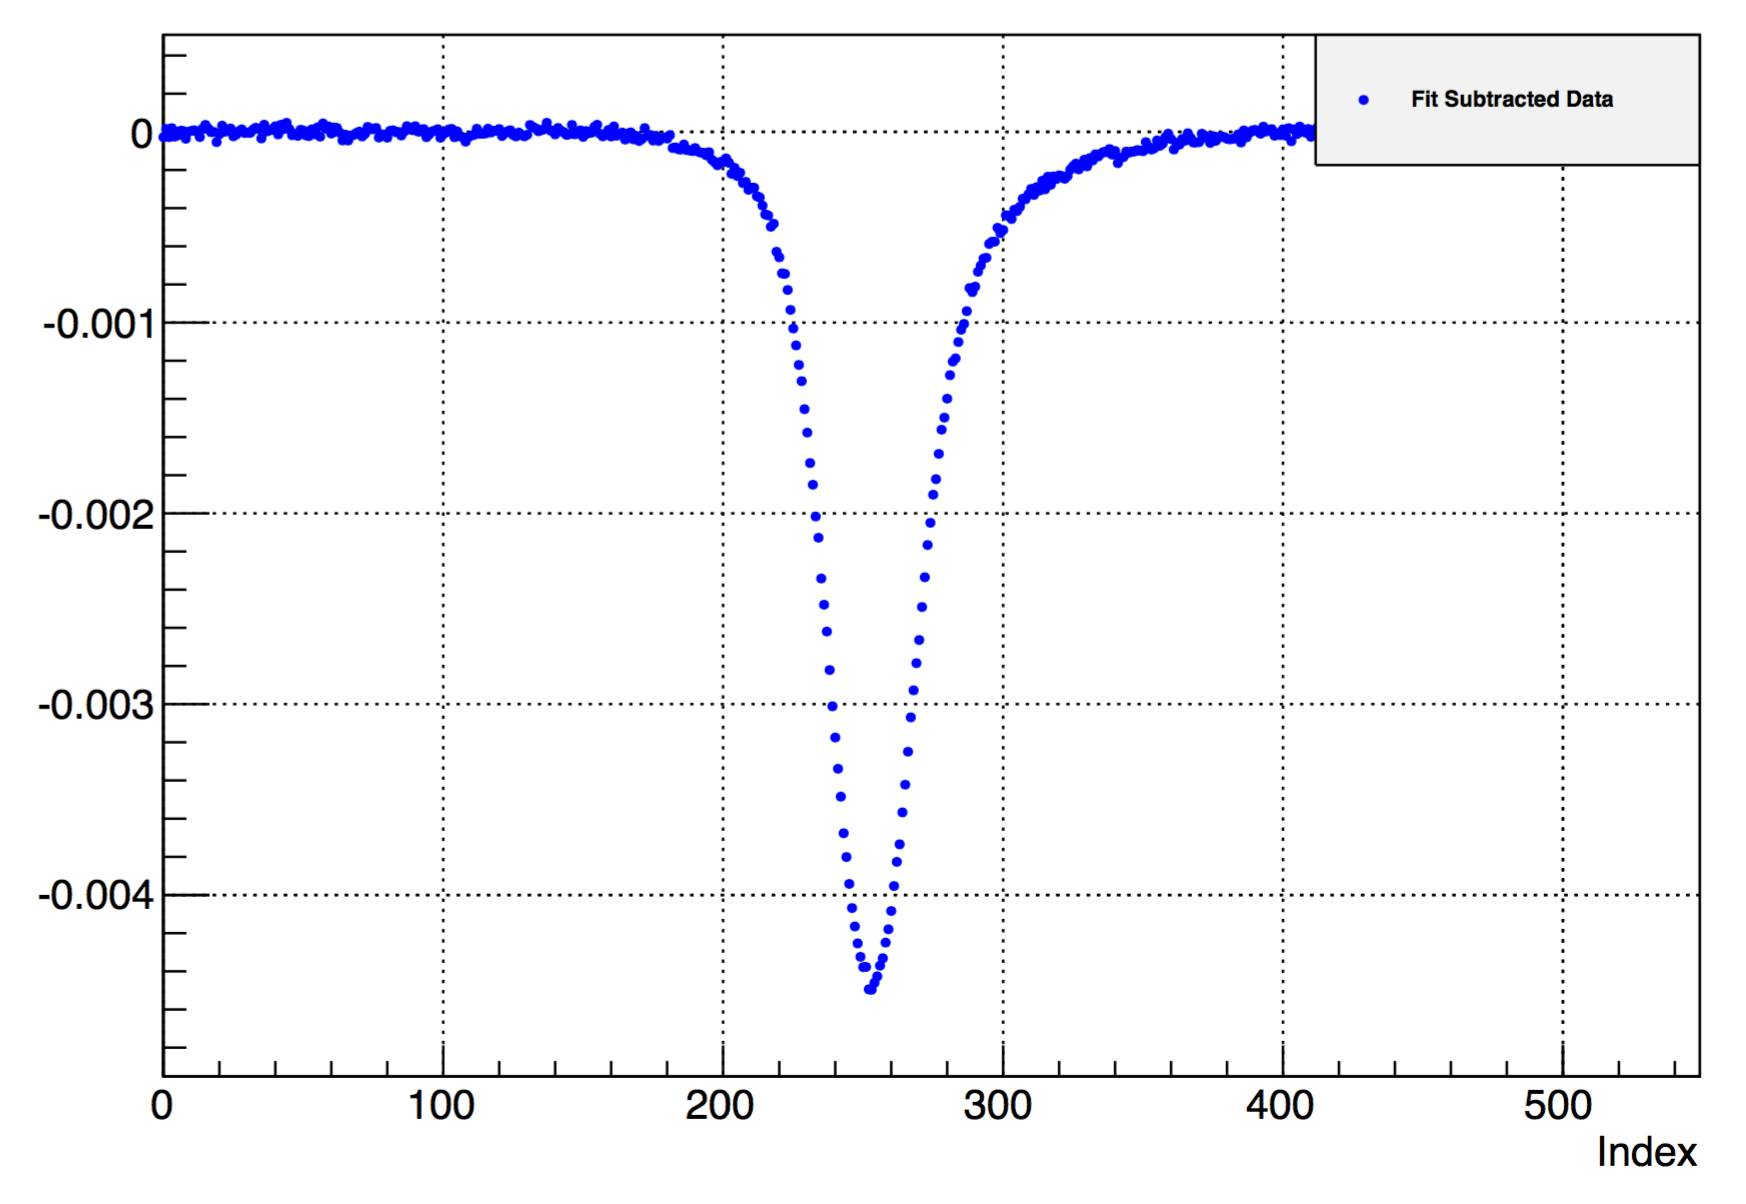
\includegraphics[width=\textwidth]{figs/target-NMR-signal.png}
    \caption{NMR signal after the subtraction. \label{C5S3SS3F1b}}
  \end{subfigure}
  \caption[Target NMR signals.]{An example of the target NMR signals. The $x$-axis index is proportional to the frequency of the RF generator. \label{C5S3SS3F1}}
\end{figure}

\begin{figure}[p!]
  \centering
  \begin{subfigure}[t]{0.9\textwidth}
    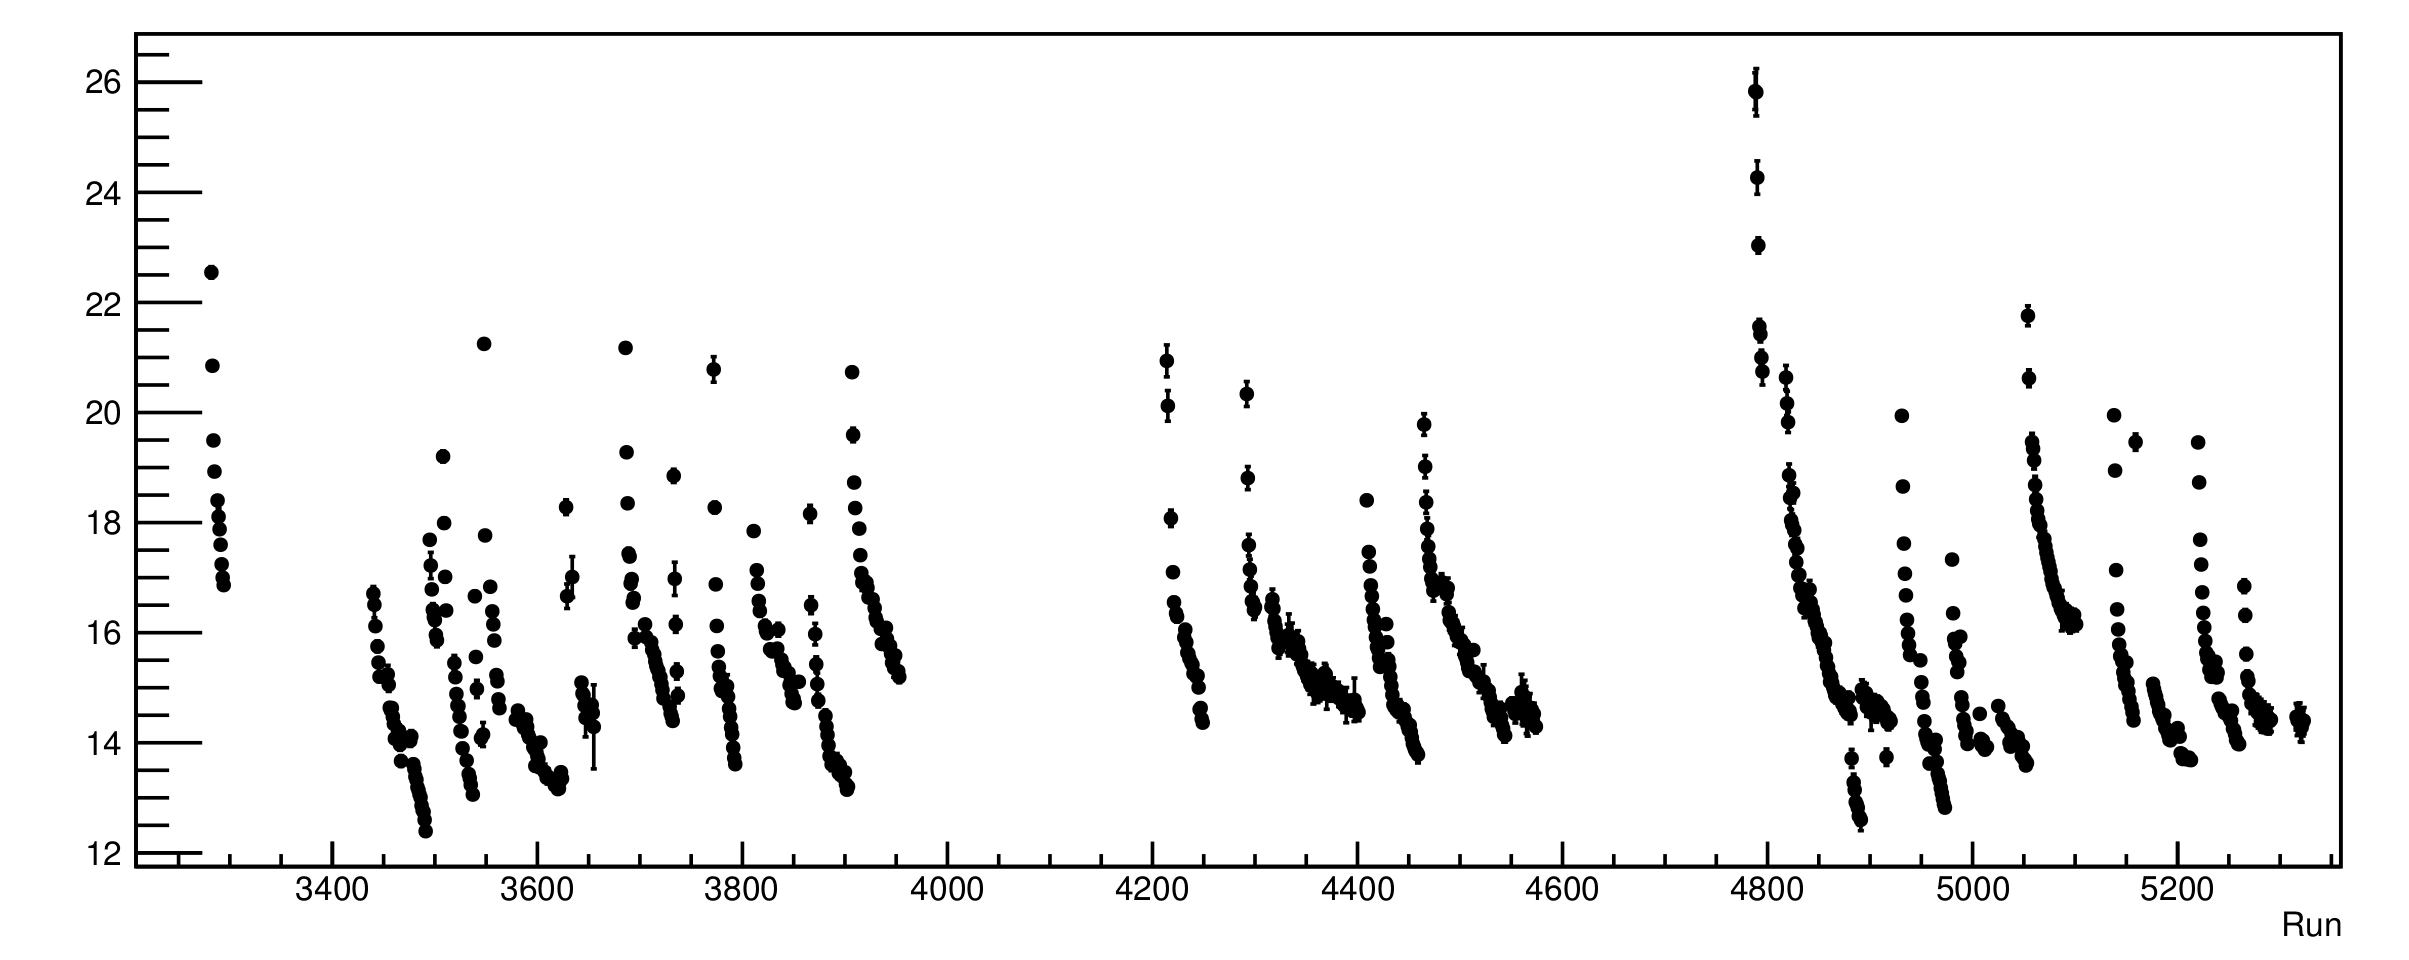
\includegraphics[width=\textwidth]{figs/target-polarization-25.png}
    \caption{2.5T target field configuration. \label{C5S3SS3F2a}}
  \end{subfigure}
  \begin{subfigure}[t]{0.9\textwidth}
    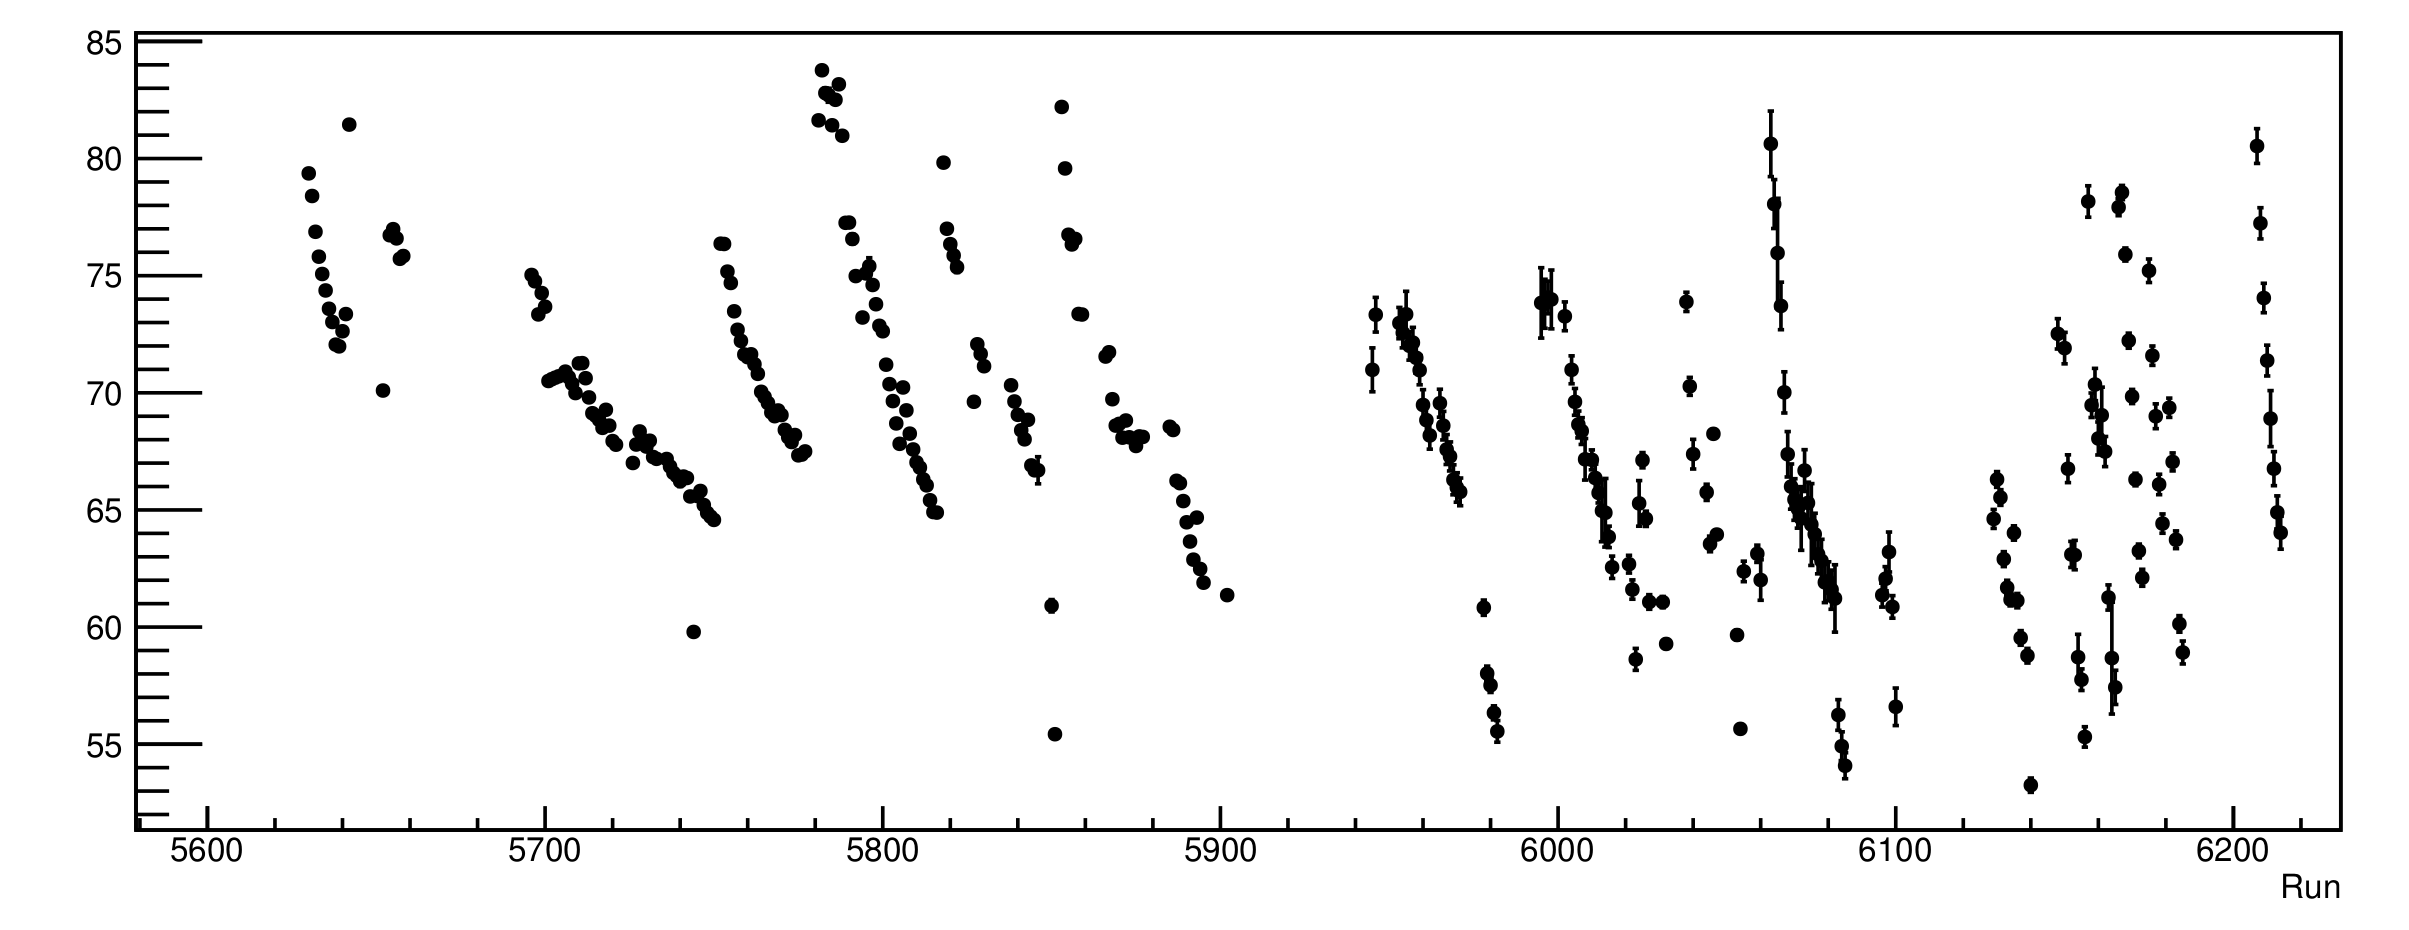
\includegraphics[width=\textwidth]{figs/target-polarization-50.png}
    \caption{5.0T target field configuration. \label{C5S3SS3F2b}}
  \end{subfigure}
  \caption[Target polarization results.]{Target polarization results during the experiment. Plot reproduced from \cite{Badman2013}. \label{C5S3SS3F2}}
\end{figure}

The output complex voltage $V(\omega,\chi)$ is proportional to the impedance of the circuit (\cref{C5S3SS3E2}). The NMR signal is composed with $V(\omega,\chi)$, together with the $Q$-meter response in the absence of $\chi$, $V(\omega,0)$, which is always referred as the ``$Q$-curve''. The $Q$-curve is measured by setting the target field so that the Larmor frequency is outside the range of the frequency scan of the $Q$-meter. The two signals are subtracted and the real part of the voltage is selected out by electronics, which gives the NMR signal $S(\omega)$:
\begin{equation} \label{C5S3SS3E3}
S(\omega) = \Re[V(\omega,\chi)-V(\omega,0)]\approx\chi''(\omega).
\end{equation}
Combining \cref{C5S3SS1E2,C5S3SS3E1,C5S3SS3E3}, the polarization $P$ can be calibrated in terms of the thermal polarization $P_{\mathrm{TE}}$ and the ratio of the integral of two NMR signals $S_{\mathrm{TE}}$ and $S_{\mathrm{enh}}$, where $S_{\mathrm{TE}}$ is the NMR signal at thermal equilibrium and $S_{\mathrm{enh}}$ is the NMR signal under microwave irradiation (when the target is polarized):
\begin{equation} \label{C5S3SS3E4}
P = \frac{\int_0^\infty S_{\mathrm{enh}}(\omega)\dd{\omega}}{\int_0^\infty S_{\mathrm{TE}}(\omega)\dd{\omega}}P_{\mathrm{TE}}.
\end{equation}
\Cref{C5S3SS3F1} shows the raw voltage signal and the NMR signal.

The $S_{\mathrm{TE}}$ curve is measured several times during the experiment, which is referred to as the TE measurement. For each different NH${}_3$ sample, the numbers of the TE measurements varied from 1 to 8 measurements, depending on the time available. The polarization was then calculated via \cref{C5S3SS3E4} on a run-by-run basis. \Cref{C5S3SS3F2} shows the final polarization results. An average polarization of 70\% and 15\% was seen for the 5.0 T and 2.5 T configurations of the target field, respectively.

The uncertainty of the polarization measurement arises from two major reasons. One is the uncertainty of the NMR signal. The other one is the uncertainty in the magnetic field and temperature readings, which contribute to the $P_{\mathrm{TE}}$ polarization calculation. The target polarization uncertainty is still being finalized. The current result is that the relative uncertainty of the target polarization is $\approx$1.2\% for the NH${}_3$ samples with 8 TE measurements, which is the best case. For the worst case with only one TE measurement, the relative uncertainty of the target polarization is $\approx$3.0\% \cite{Badman2013}.

\section{Hall A High Resolution Spectrometers}
\label{C5S4}

E08-027 uses the two standard Hall A high resolution spectrometers (HRS) to detect the scattered electrons \cite{Alcorn2004}. The two HRSs are nearly identical, and are referred to as HRS-L (left arm) and HRS-R (right arm) respectively. The main characteristics of HRS are summarized in \Cref{C5S4T1}. Both arms contain three quadrupoles and a dipole magnet in a QQDQ configuration as illustrated in \Cref{C5S4F1}. The Q1, Q2 and Q3 are three superconducting quadrupoles to provide focusing: Q1 focuses in the vertical plane and Q2 and Q3 in the transverse plane. The momentum of the electrons that reach the detector package are determined by the superconducting dipole with a momentum resolution at the $10^{-4}$ level. The electrons are bent by the dipole magnet by an angle of \SI{45}{\degree} in the vertical direction.

\begin{figure}[p!]
  \centering
  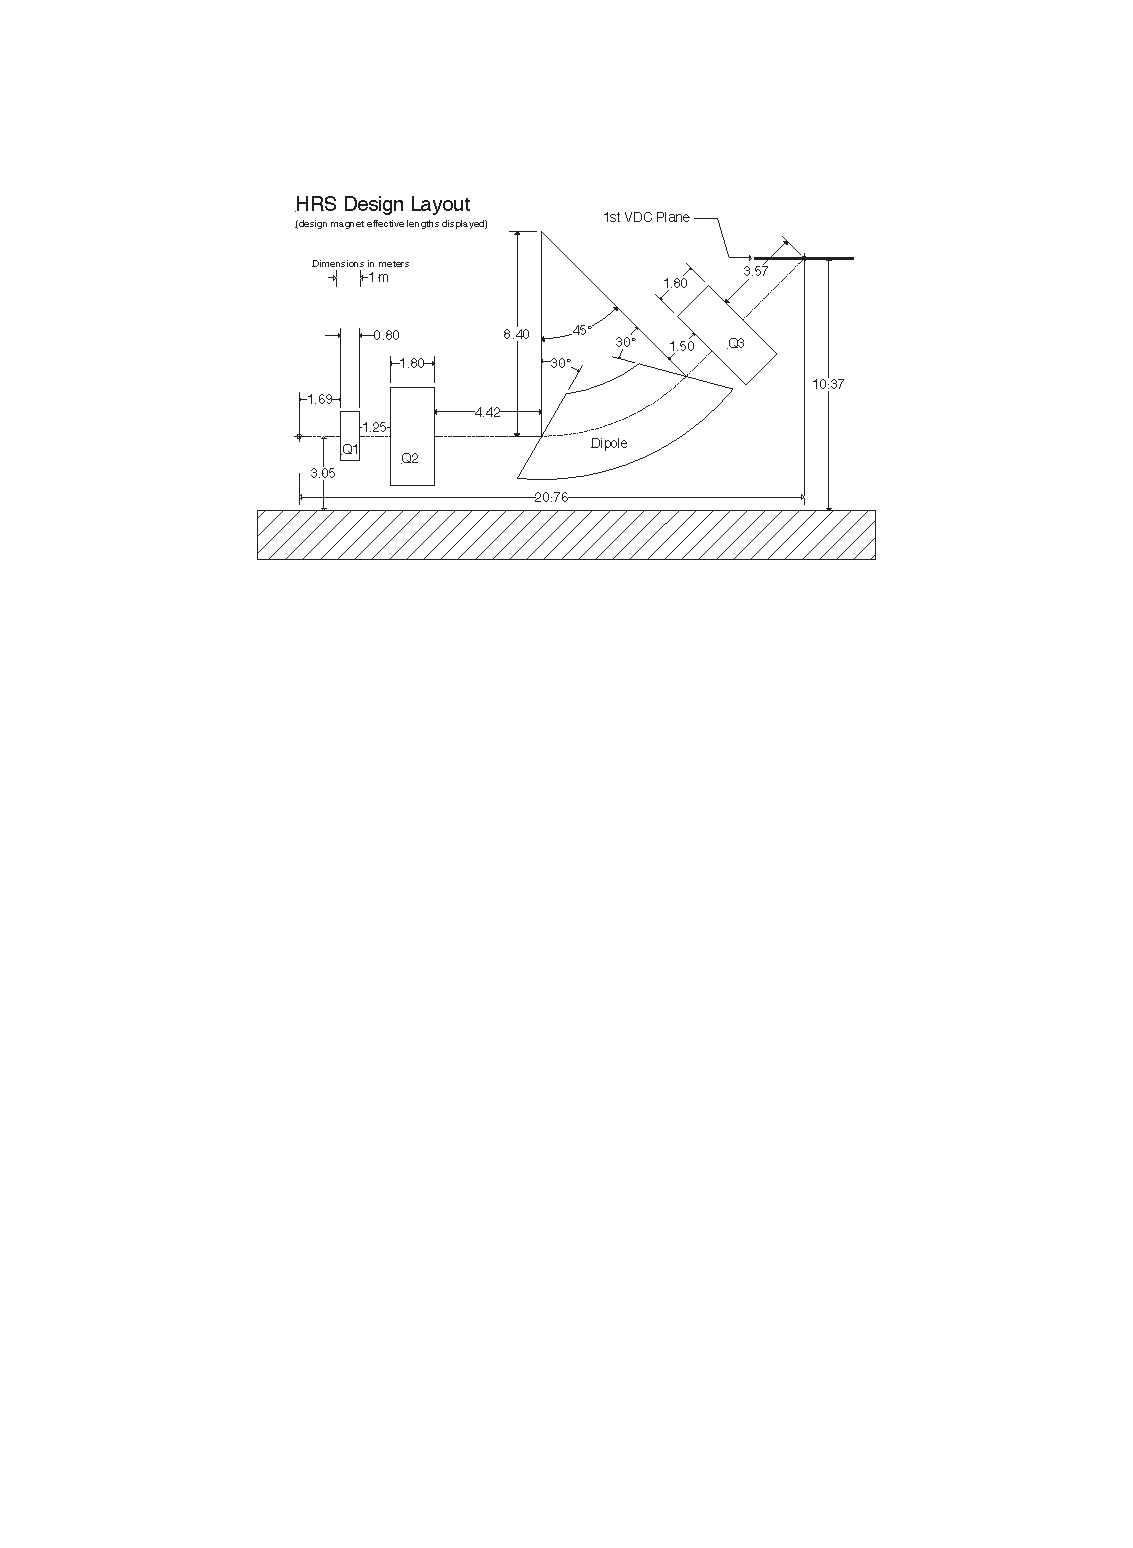
\includegraphics[width=\textwidth]{figs/HRS.pdf}
  \caption[Magnet configuration for HRS.]{Magnet configuration for HRS. Also shown is the location of the first VDC tracking detector. Figure reproduced from \cite{Alcorn2004}. \label{C5S4F1}}
\end{figure}

\begin{table}[p!]
  \centering
  \begin{tabular}{|l|c|}
    \hline\hline
    Bending angle & \SI{45}{\degree} \\ \hline
    Optical length & 23.4 m \\ \hline
    Momentum range & 0.3$\sim$4.0 GeV/c \\ \hline
    Momentum acceptance & $\pm$4.5\% \\ \hline
    Momentum resolution & $1\times10^{-4}$ \\ \hline
    Angular range (HRS-L) & \SI{12.5}{\degree}$\sim$\SI{150}{\degree} \\ \hline
    Angular range (HRS-R) & \SI{12.5}{\degree}$\sim$\SI{130}{\degree} \\ \hline
    Angular acceptance (horizontal) & $\pm$30 mrad \\ \hline
    Angular acceptance (vertical) & $\pm$60 mrad \\ \hline
    Angular resolution (horizontal) & 0.5 mrad \\ \hline
    Angular resolution (vertical) & 1.0 mrad \\ \hline
    Solid angle at $\delta=0$, $y_0=0$ & 6 msr \\ \hline
    Transverse length acceptance & $\pm$5 cm \\ \hline
    Transverse position resolution & 1 mm \\ \hline
  \end{tabular}
  \caption[The characteristics of the HRS.]{The characteristics of the standard Hall A spectrometers. Table reproduced from \cite{Alcorn2004}. \label{C5S4T1}}
\end{table}

\subsection{Septum Magnet}
\label{C5S4SS1}

E08-027 measured the scattered electrons at an angle of $\approx$\SI{5.77}{\degree}. However, the HRS have a minimum achievable angle of \SI{12.5}{\degree}, that is mainly because the Q1 magnet would hit the beam pipe if the spectrometer is moved to a smaller angle. During the experiment, a pair of septum magnets was used to allow both spectrometers to reach angles down to \SI{5.77}{\degree} \cite{G2P}. The septum magnet pair was located in front of the Q1 entrence of the HRS and horizontally bent the electrons with scattering angle $\approx$\SI{5.77}{\degree} into the spectrometer located at \SI{12.5}{\degree}. The coils of the septum magnet burned twice during the experiment, which led to three different septum configurations. The detailed configurations are listed in \Cref{C5T1}.

\subsection{Detector Package}
\label{C5S4SS2}

\begin{figure}[b!]
  \centering
  \begin{subfigure}[t]{0.49\textwidth}
    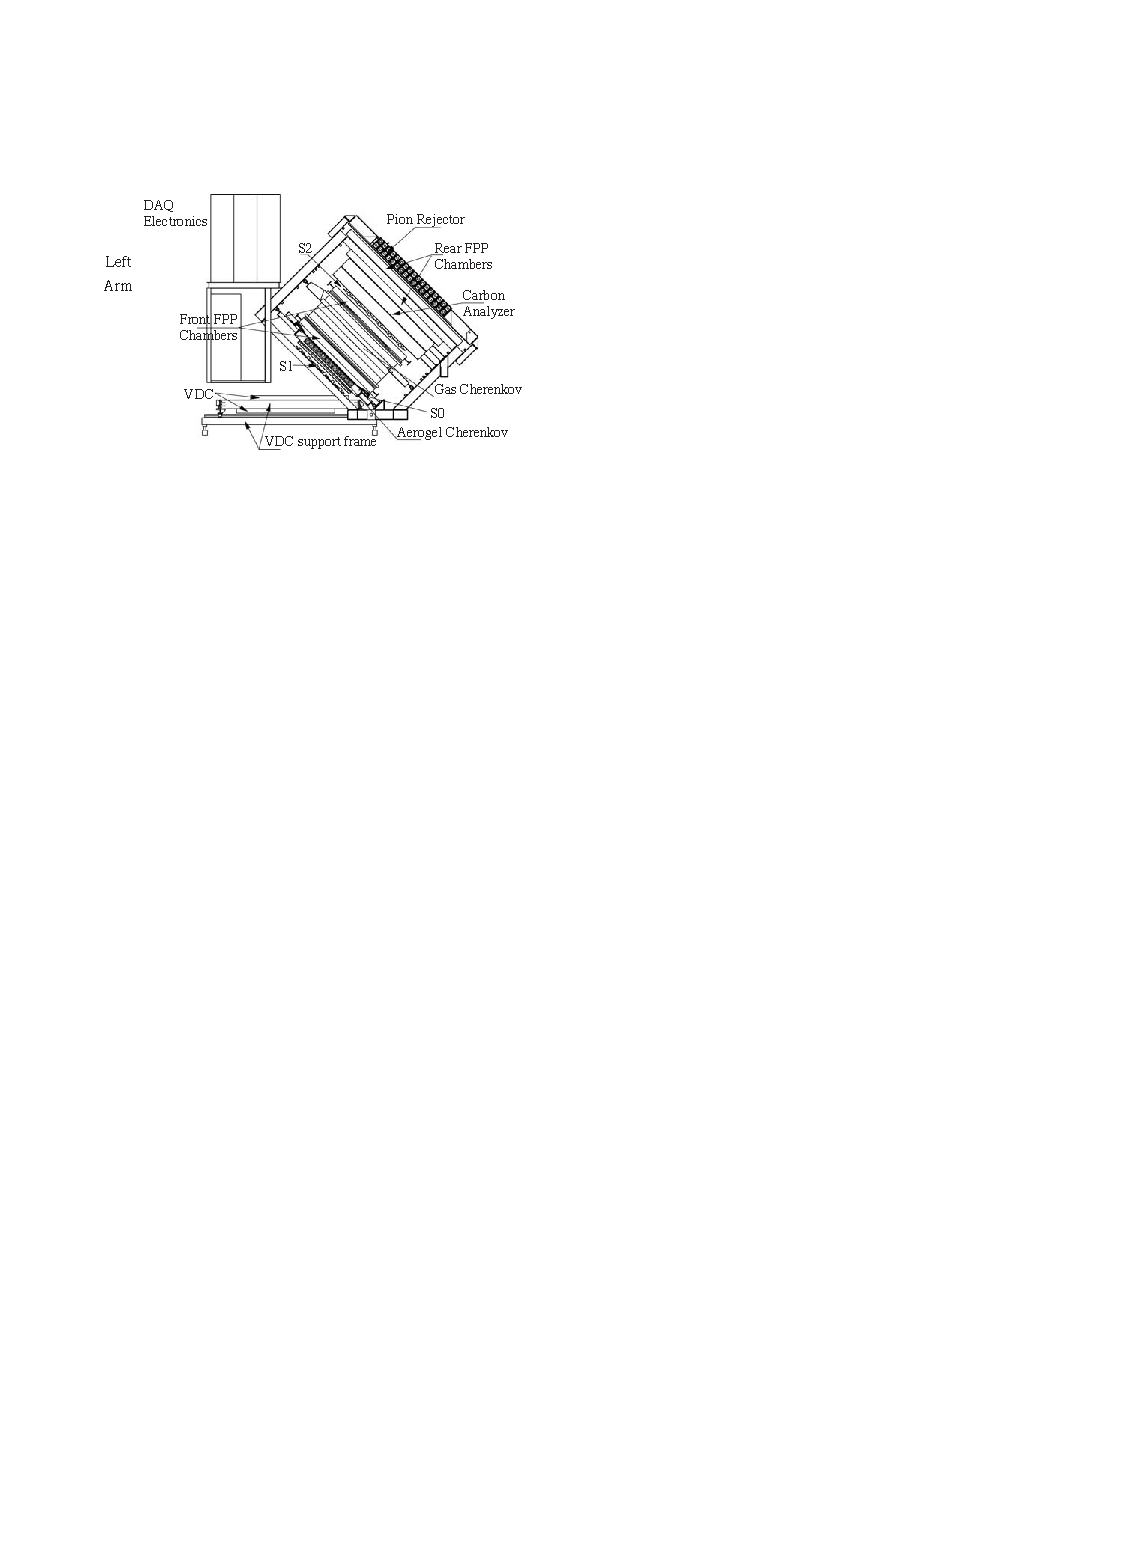
\includegraphics[width=\textwidth]{figs/detector-package-left.pdf}
    \caption{Left arm. \label{C5S4SS2F1a}}
  \end{subfigure}
  \begin{subfigure}[t]{0.49\textwidth}
    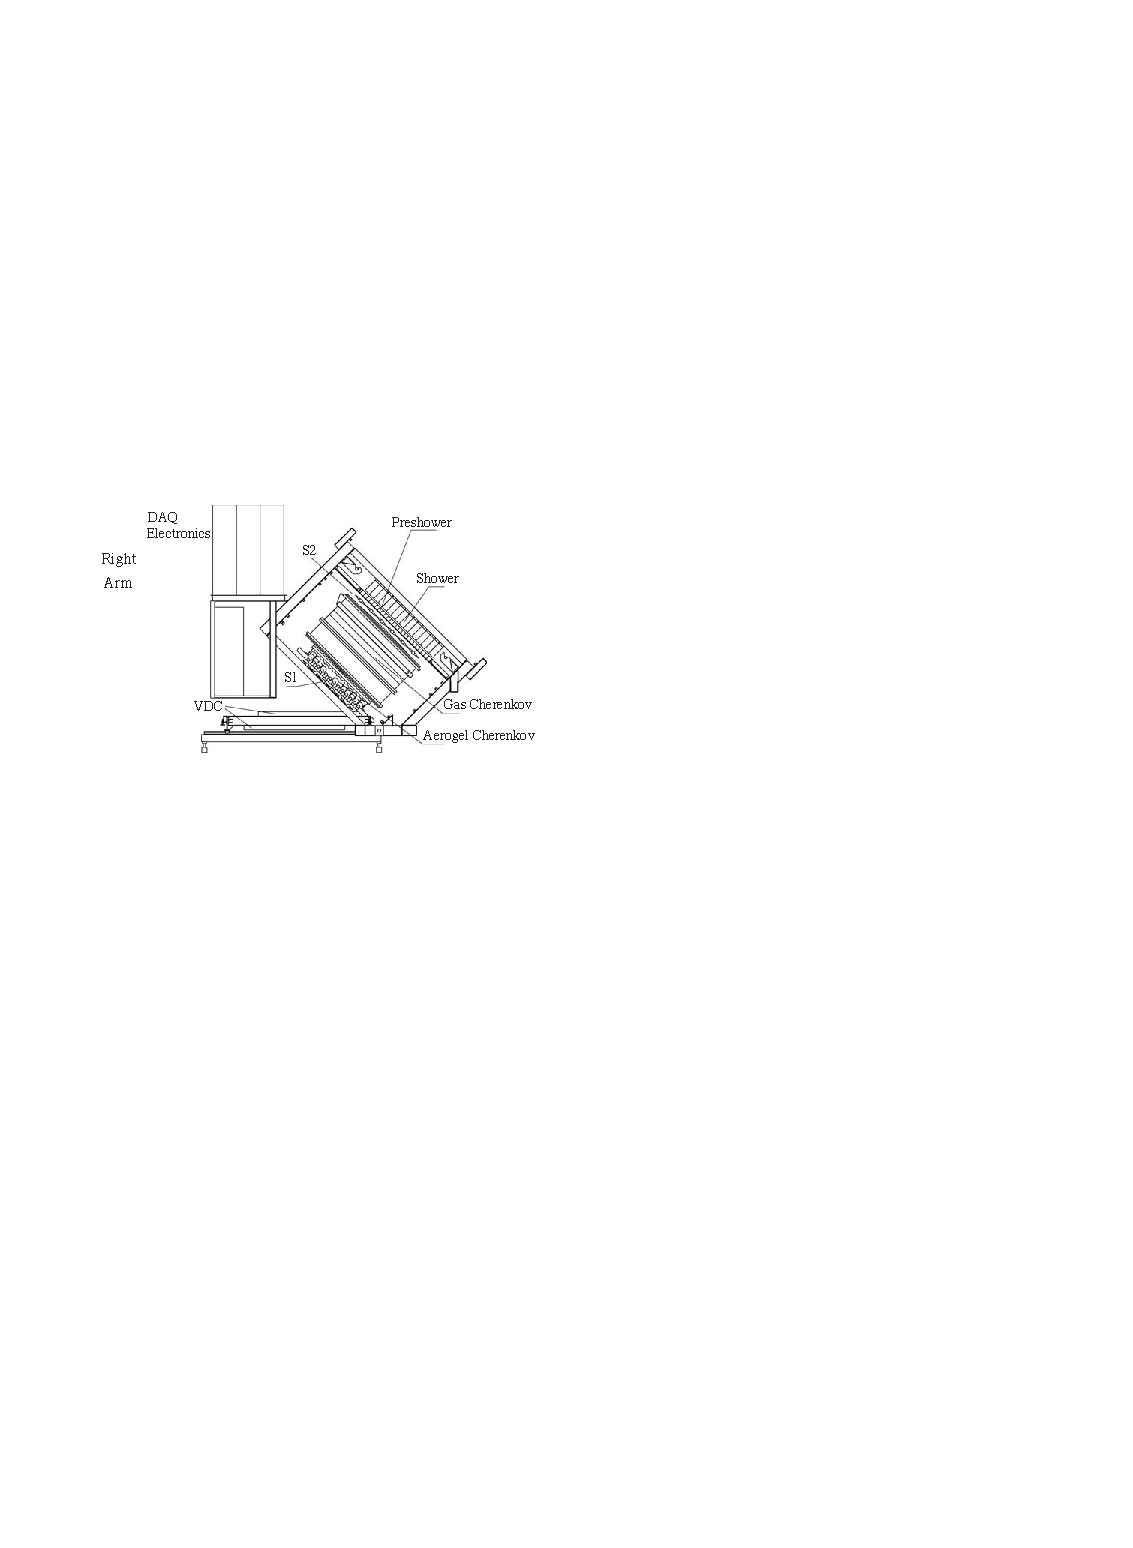
\includegraphics[width=\textwidth]{figs/detector-package-right.pdf}
    \caption{Right arm. \label{C5S4SS2F1b}}
  \end{subfigure}
  \caption[Detector package of HRS.]{Detector package of HRS. Note that only the VDC, scintillators (S1 and S2), gas Cherenkov detector and the calorimeters (pion rejectors in HRS-L, shower and pre-shower in HRS-R) were used during E08-027. Figure reproduced from \cite{Alcorn2004}. \label{C5S4SS2F1}}
\end{figure}

The detector package of the HRS is in a shielding hut together with the DAQ electronics at the end of the magnet group. The standard layout of the detector package is shown in \Cref{C5S4SS2F1}. The trajectory and the momentum of the scattered particle is determined by a pair of vertical drift chambers. Then the particles pass through a pair of plastic scintillator planes which generate the trigger for DAQ system. A gas Cherenkov detector and a set of lead glass calorimeters (pion rejectors in HRS-L, shower and pre-shower in HRS-R) are used for particle identification (PID). The main difference between the two arms is in the second layer of the calorimeters. The lead-glass blocks are aligned perpendicular to the particle trajectories in the left arm, whereas in the right arm the blocks in the second layer are oriented parallel to the trajectories.

\subsubsection{Vertical Drift Chambers}

The vertical drift chambers (VDC) in each spectrometer consists of two VDC chambers, each composed of two wire planes in a UV configuration \cite{Fissum2001} as shown in \Cref{C5S4SS2F2}. The U and V planes are orthogonal and lie in the laboratory horizontal plane. They are inclined at an angle of \SI{45}{\degree} with respect to the dispersive direction of the dipole. Each plane contains 368 sense wires, spaced 4.24 mm apart. The upper and lower VDC chambers are separated by about 335 mm. The spectrometer focal plane is referred as the first wire plane (U1) that the particles traverse through. The concept of the focal plane is important to the spectrometer optics study which will be discussed in detail in \Cref{C6}.

\begin{figure}[b!]
  \centering
  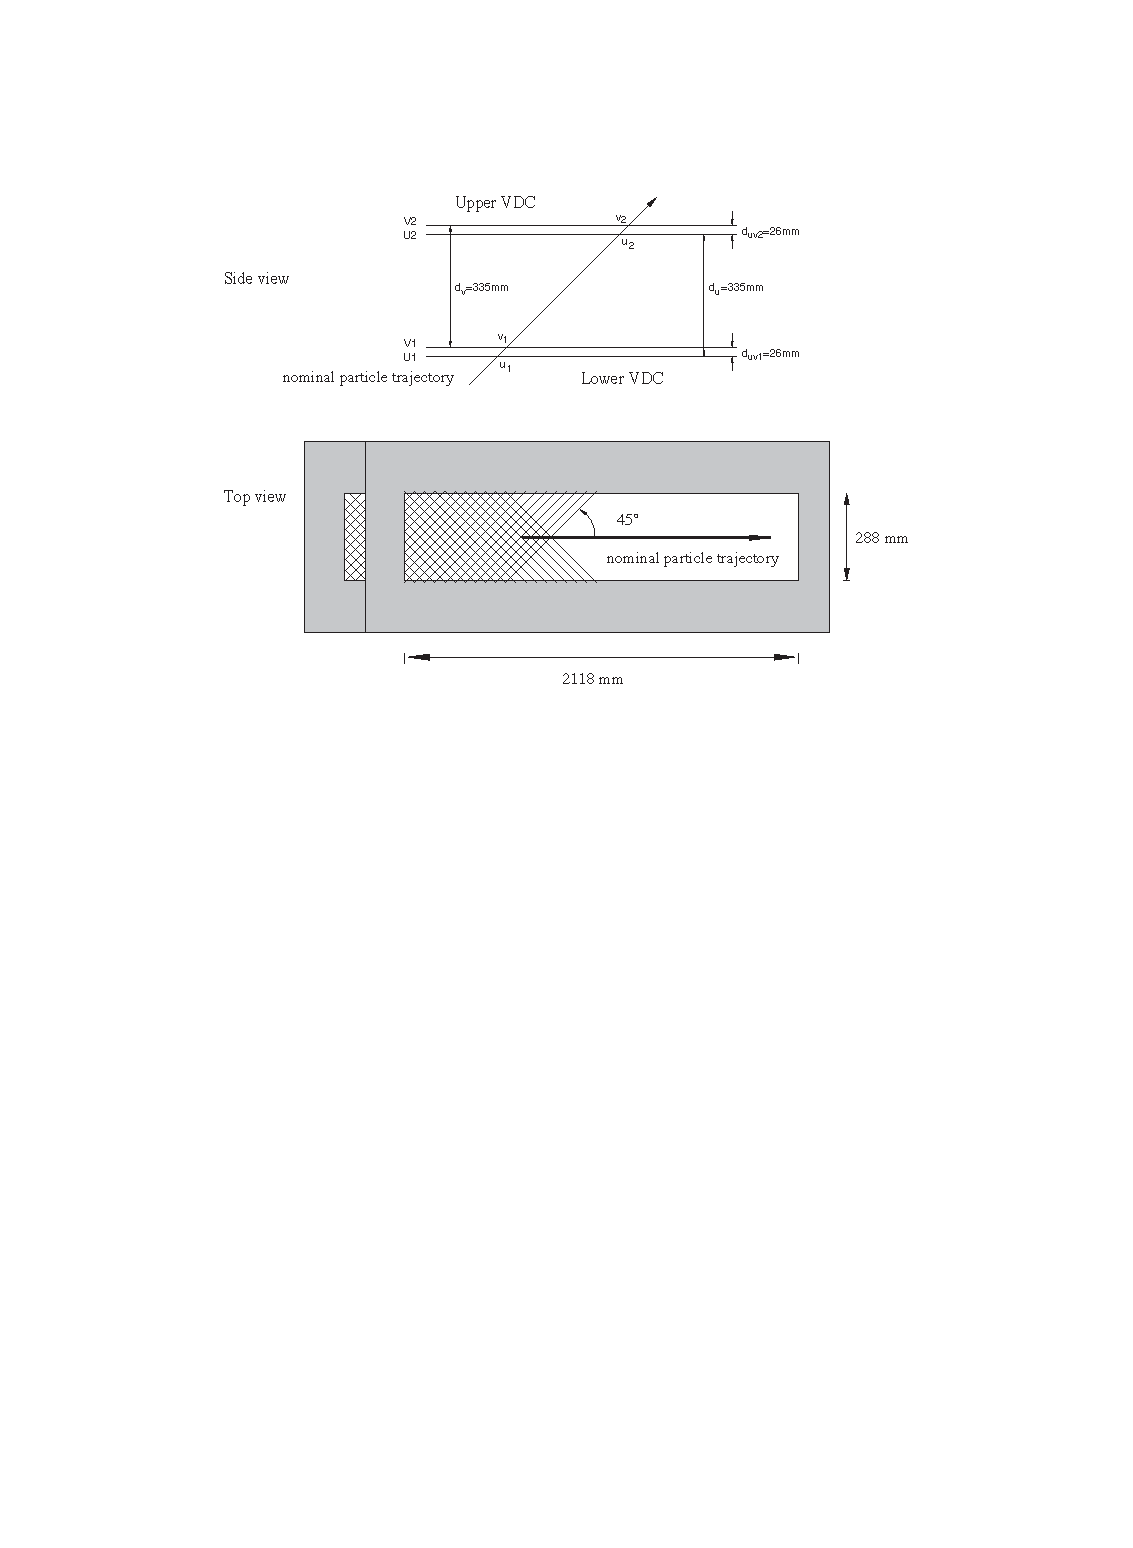
\includegraphics[width=0.75\textwidth]{figs/VDC.pdf}
  \caption[Schematic diagram of the Hall A vertical drift chambers.]{Schematic diagram of the Hall A vertical drift chambers. Plot reproduced from \cite{Alcorn2004}. \label{C5S4SS2F2}}
\end{figure}

The chambers are filled with a gas mixture of argon (62\%) and ethane (38\%). Argon provides the ionizing medium while ethane absorbs the photons produced from ionization. The electric field of the VDCs is shaped by gold-plated mylar planes powered at -4 kV. Ionized electrons drift along the electric field lines and rapidly accelerate towards the wire when they are close to a wire, producing a shower of secondary ionizations. The approaching avalanche of electrons induces a signal on the wire.

By design, the electrons that travel across the VDCs with an angle of \SI{45}{\degree} will fire four to six wires per plane. This provides an accurate reconstruction of the particle's trajectory. The trajectories are reconstructed with the timing information provided by time-to-digital converters (TDCs) which are connected to the wires. The timing information can be used to determine the drift distance for each wire. The cross-over point is then determined via a linear fit of drift distances versus the wire position. The position and angular resolution of the focal plane are approximately 100 $\mu$m and 0.5 mrad, respectively.

\subsubsection{Scintillator Planes}

Two plastic scintillator planes (S1 and S2m) separated by 2 m are used to form the trigger for the DAQ system. Both planes are made of overlapping paddles of plastic scintillators \cite{Alcorn2004}. The S1 plane has 6 paddles and the S2m plane consists of 12 paddles. Each paddle is monitored by a pair of photomultiplier tubes (PMTs), one at each end. The timing resolution for each plane is about 0.3 ns.

The main trigger (referred as T3 for HRS-L and T1 for HRS-R) is formed as:
\begin{itemize}[parsep=0pt]
\item A paddle in S1 is defined to be fired if there are signals from both its left and right PMTs;
\item A paddle in S2m is defined to be fired if there are signals from both its left and right PMTs;
\item One S1 paddle and one S2m paddle are both fired within a specified timing window.
\end{itemize}
A secondary trigger (referred as T4 and T2 for left and right arm, respectively) is used to monitor the scintillator efficiency. The efficiency trigger is exclusive to T1(or T3) trigger and is formed by requiring either one S1 paddle or one S2m paddle to be fired as well as a signal from the gas Cherenkov detector. The T2 and T4 triggers represent possibly good events but one of the scintillator planes failed to detect.

The triggers are sent to the trigger supervisor (TS) to determine if the event should be sent to the DAQ system. The DAQ has a deadtime and cannot record every event if the event rate is high. The fraction of events which the DAQ records is called the livetime $LT$, which is determined by the deadtime $DT$ as $LT=1-DT$. The DAQ deadtime can be decreased by scaling the incoming events with a prescale factor $ps$ at the TS which means that only 1 of every $ps$ events fed to the TS is sent to the DAQ system. The livetime depends on the event type and helicity state. It can be calculated by the number of triggers accepted by the DAQ system, $NT_{\mathrm{acc}}$, and the total number of triggers input to the TS, $NT$,  which is recorded by scalers (The scalers are treated as deadtime-less):
\begin{equation} \label{C5S4SS2E1}
LT^{\pm} = \frac{ps\cdot NT_{\mathrm{acc}}^{\pm}}{NT},
\end{equation}

\begin{figure}[tb!]
  \centering
  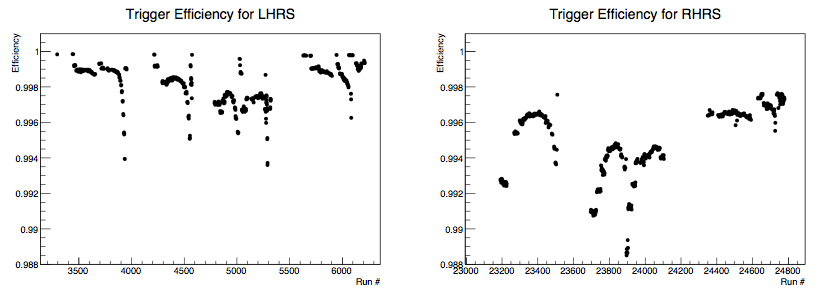
\includegraphics[width=\textwidth]{figs/trigger-efficiency.png}
  \caption[Trigger efficiencies of HRS.]{Trigger efficiencies of HRS, calculated using \cref{C5S4SS2E2}. Plot reproduced from \cite{Zielinski2014a}. \label{C5S4SS2F3}}
\end{figure}

The trigger efficiency $\eta_{\mathrm{T}}$ is defined as:
\begin{equation} \label{C5S4SS2E2}
\eta_{\mathrm{T}} = \frac{NT_{\mathrm{main}}}{NT_{\mathrm{main}}+NT_{\mathrm{eff}}},
\end{equation}
where the $NT_{\mathrm{main}}$ are the total number of the T1 (or T3) trigger and $NT_{\mathrm{eff}}$ are the total number of the T2 (or T4) trigger described above. The trigger efficiency results are shown in \Cref{C5S4SS2F3}. Overall, the efficiencies are greater than 99.1\% \cite{Zielinski2014a}. Some substructure can be seen in the data, for example, the trigger efficiency at lower momenta tends to drop off. However, it is still safe to conclude that the correction to the cross-sections from the trigger efficiency is less than 1\%.

\subsubsection{Gas Cherenkov Detector}

The speed of light in a medium is always lower than the speed of light in vacuum. The ratio between the two speeds is the index of refraction ($n$), which is a characteristic of the medium. Although the speed of light in the vacuum is the upper limit of the velocity of a particle, the velocity of a high energy particle may exceed the speed of light in a medium, $v>c/n$. A charged particle disrupts the local electromagnetic field when it travels through the medium. When the particle is traveling fast enough, the disturbance accumulates in the medium due to the limited response speed (speed of light in the medium), thus the energy contained in this disturbance radiates as a coherent shockwave, known as Cherenkov radiation \cite{Leo1994}. The wave is emitted in a cone. \Cref{C5S4SS2F4} shows the geometry of the Cherenkov radiation. The threshold for the production of Cherenkov radiation is given by:
\begin{equation} \label{C5S4SS2E3}
\beta c \geq\frac{c}{n},
\end{equation}
where $\beta=v/c$ is the velocity of the particle in unit of $c$. Since the speed threshold to produce Cherenkov radiation is $\beta\geq1/n$, the momentum threshold is therefore dependent on the mass of the particle:
\begin{equation} \label{C5S4SS2E4}
p_{\mathrm{thr}} = m_0\gamma v = m_0\frac{c}{\sqrt{n^2-1}}.
\end{equation}

\begin{figure}[tb!]
  \centering
  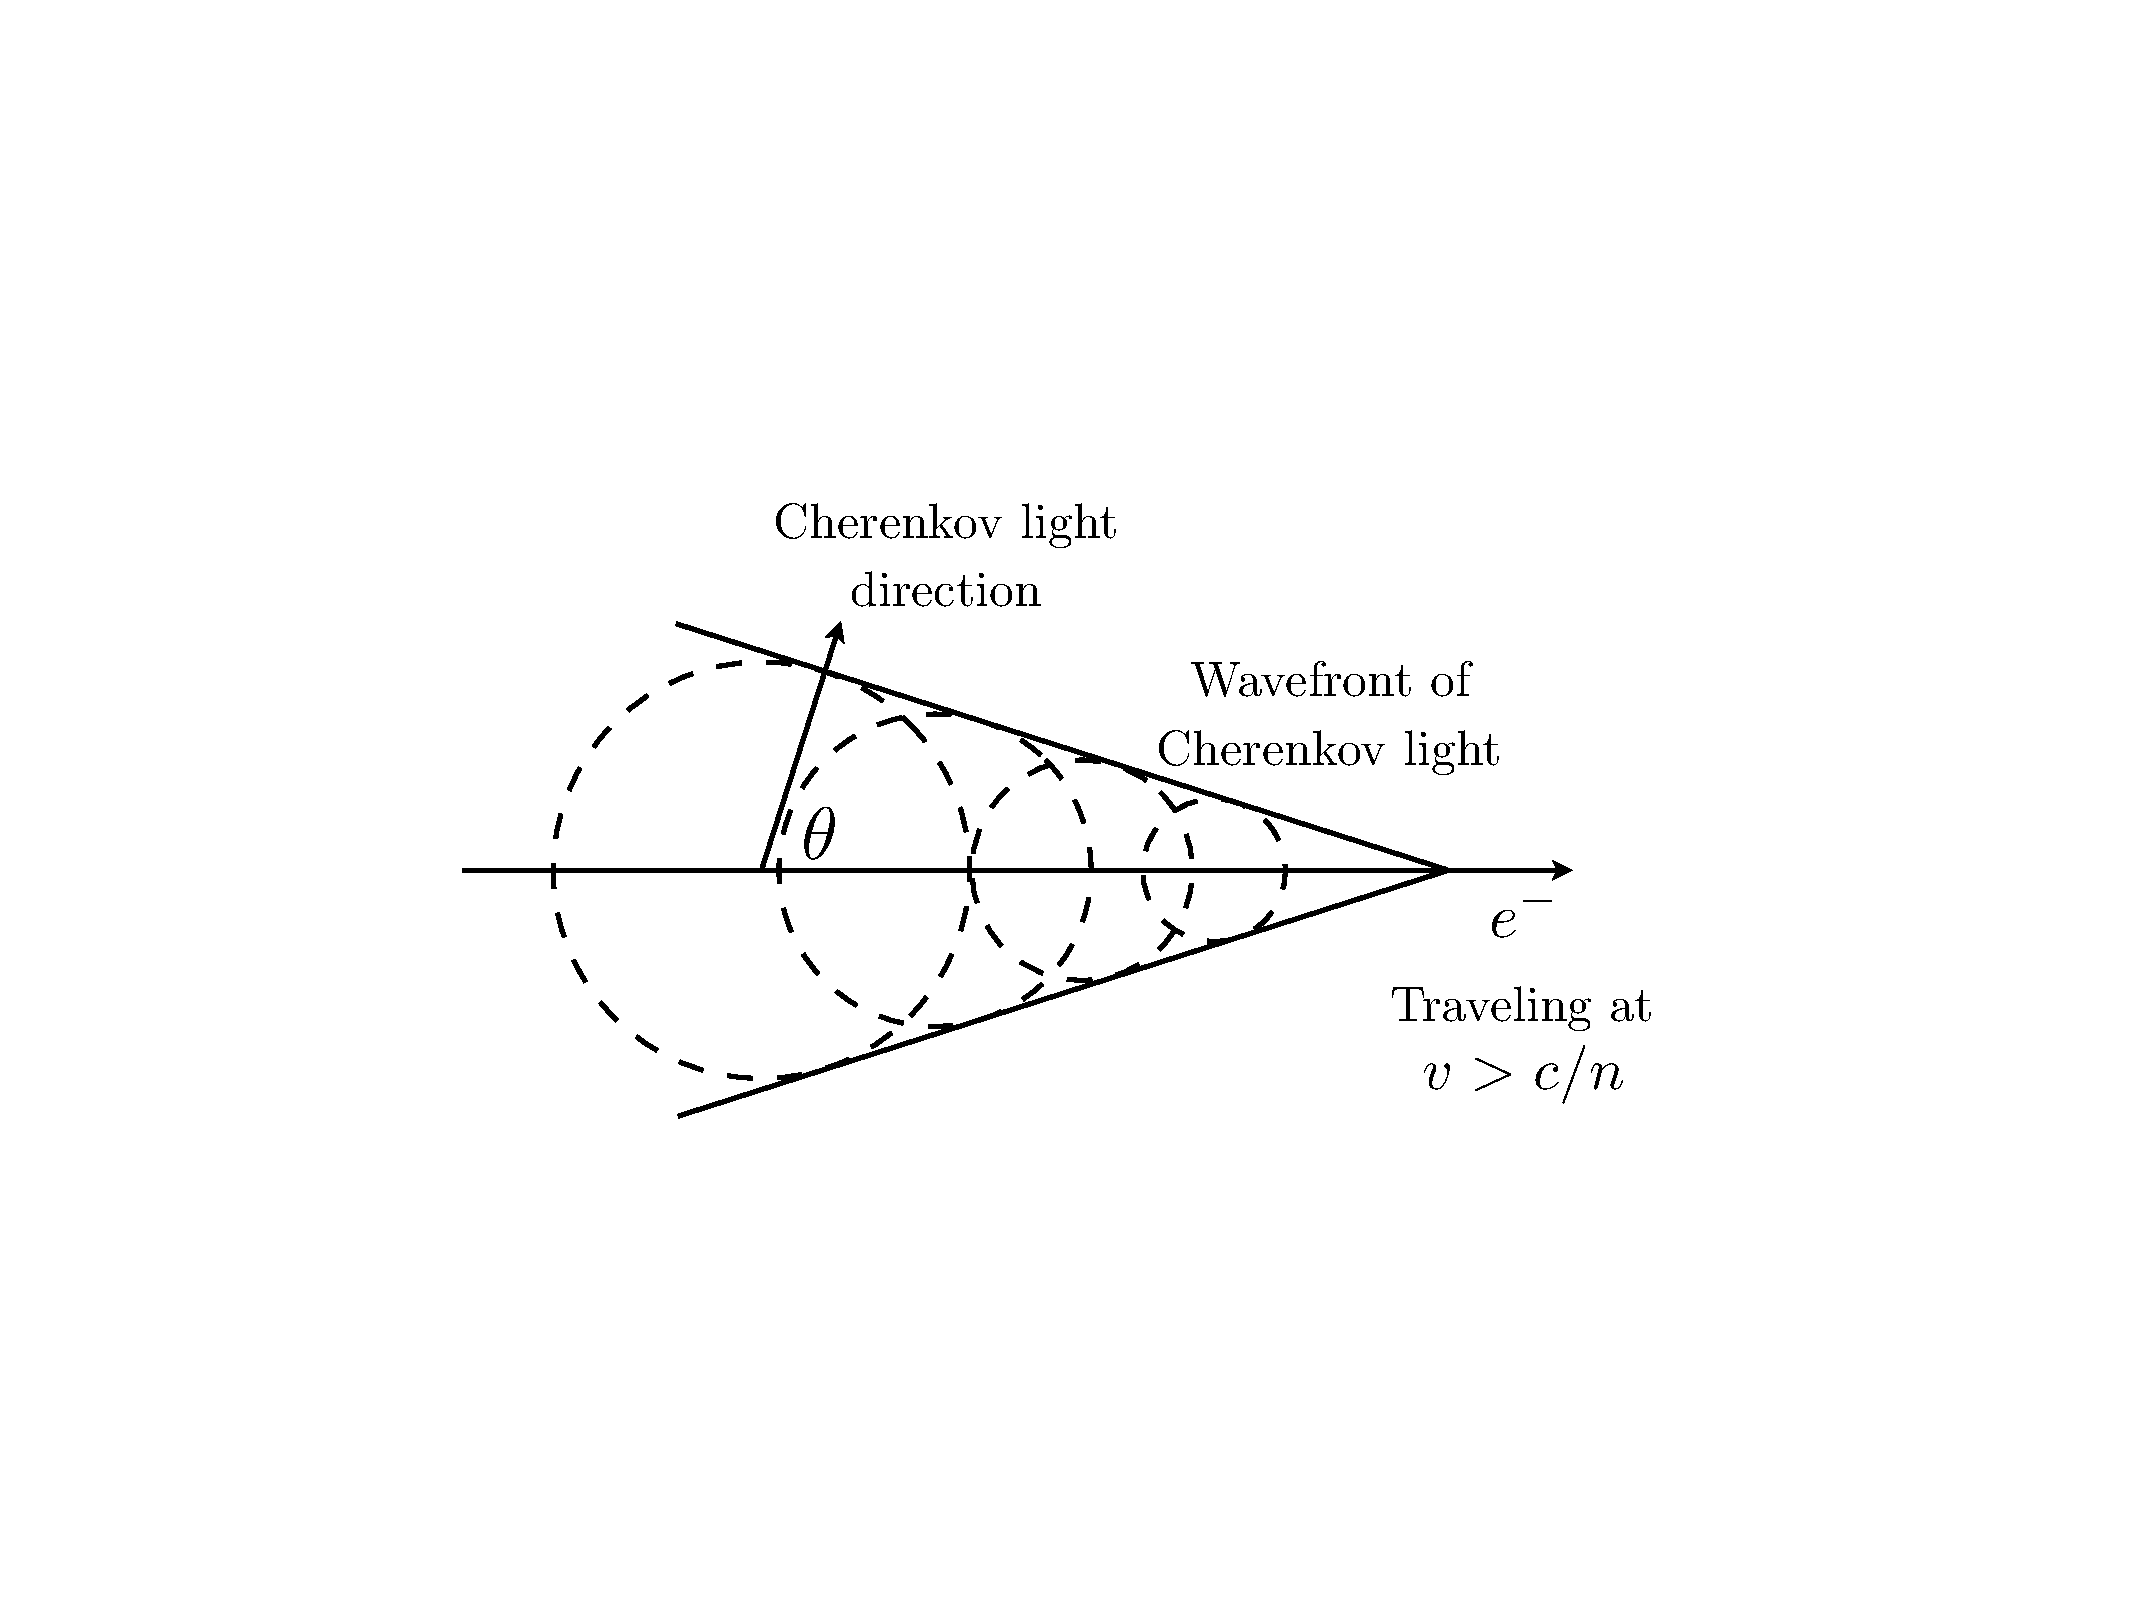
\includegraphics[width=0.6\textwidth]{figs/Cherenkov-radiation.pdf}
  \caption[Geometry of the Cherenkov radiation.]{Geometry of the Cherenkov radiation. The angle $\theta$ is given by $\cos\theta=1/n\beta$. \label{C5S4SS2F4}}
\end{figure}

In the detector package of HRS, a gas Cherenkov detector \cite{Iodice1998} is sandwiched between the two scintillator planes. The detector is filled with carbon dioxide gas with index of refraction $n=1.00041$. From \cref{C5S4SS2E4}, the momentum threshold for electrons is 0.018 GeV/c, whereas the threshold for pions is 4.87 GeV/c. Thus, the Cherenkov detector can be used to identify the electrons and pions for momentum between 0.018 and 4.87 GeV/c.

The detector has a path length of 1.5 m. Ten spherical mirrors are installed to focus the Cherenkov light onto 10 PMTs. The signals from the PMTs are sent to ADCs and are summed together, representing the total radiation produced by that particle. However, pions can cause a sizable background when they interact with materials in the detector causing secondary electrons. These background events are removed with the aid of a lead-glass calorimeter.

\subsubsection{Electromagnetic Calorimeter}

When a high energy particle traverses through a dense material, an electromagnetic cascade of photons and electron-positron pairs is generated \cite{Leo1994}. The light produced by the cascade is linearly proportional to the energy deposited in the material and can be detected by PMTs.

The calorimeters of the left and right arm of HRS are slightly different in construction \cite{Alcorn2004}, see \Cref{C5S4SS2F5}. The HRS-L calorimeter is composed of two layers of lead-glass blocks, each made of thirty-four blocks, oriented perpendicular to the particle trajectory. The blocks in the first layer are 14.5 cm$\times$14.5 cm$\times$30 cm while the blocks in the second layer are 14.5 cm$\times$14.5 cm$\times$35 cm. On HRS-R, the first layer of the calorimeter contains 48 10 cm$\times$10 cm$\times$35 cm lead-glass blocks which are oriented perpendicular to the particle trajectory, whereas the second layer is composed of 80 14.5 cm$\times$14.5 cm$\times$35 cm blocks which are oriented parallel to the particle trajectory. The major difference between the HRS-L and HRS-R calorimeters is that the HRS-R calorimeter is a total energy absorber, which means the scattered electrons will deposit all of their energies in the calorimeter since it is thick enough, while the HRS-L calorimeter is not a full energy absorber because of the thinner length.

\begin{figure}[tb!]
  \centering
  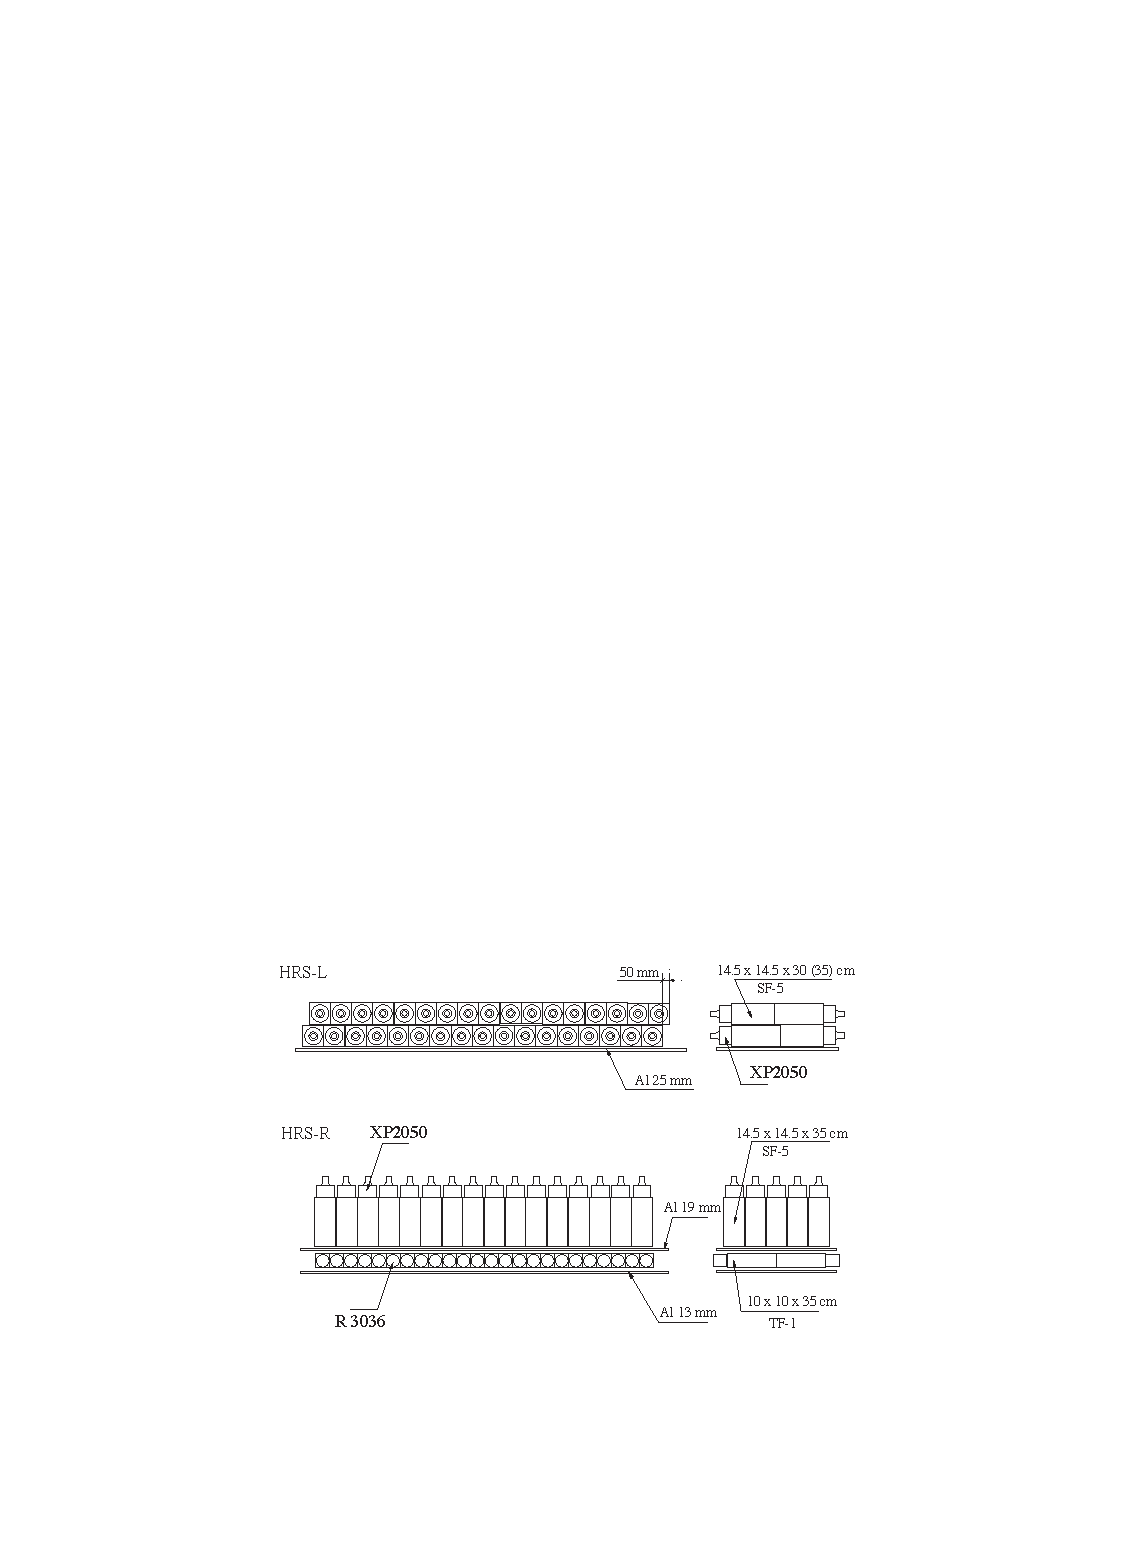
\includegraphics[width=0.8\textwidth]{figs/calorimeters.pdf}
  \caption[The electromagnetic calorimeters in the HRS.]{The electromagnetic calorimeters in the HRS. Plot reproduced from \cite{Alcorn2004}. \label{C5S4SS2F5}}
\end{figure}

%%%%%%%%%%%%%%%%%%%%%%%%%%%%%%%%%%%%%%%%%%%%%%%%%%%%%%%%%%%%%%%%%%%%%%
% -*-latex-*-
